\documentclass[12pt]{article}
\usepackage{authblk}
\usepackage[english]{babel}
\usepackage{threeparttable}
\usepackage{pdflscape}
% Bibliography Style
\usepackage[authoryear]{natbib}  % Enables Chicago author-date citations
\bibliographystyle{chicago}
\newcommand{\sym}[1]{\rlap{$^{#1}$}}
\usepackage{soul}
\usepackage{amsmath}
\usepackage{graphicx}   % Required for \resizebox{}
\usepackage[colorlinks=true, allcolors=blue]{hyperref}
\usepackage{ulem} % For \uline command

 \newcommand\citeapos[1]{\citeauthor{#1}'s (\citeyear{#1})} % use apostrofe for references e.g. Lehr's (1990)
\makeatletter
 \def\@mb@citenamelist{cite,citep,citet,citealp,citealt,citeapos} % this will add the custom made command 'citeapos' to the list of newcite commands
 \makeatother
% Margins: 1-inch all around
\usepackage[margin=1in]{geometry}

% Font: Times New Roman (or closest equivalent)
% \usepackage{times}  

% Table & Formatting Packages
\usepackage{threeparttable} % For notes below tables
\usepackage{multirow}
\usepackage{makecell}
\usepackage{array}          % Improved column alignment
\usepackage{siunitx}        % Proper numeric alignment
\usepackage{booktabs}       % Professional table formatting
\usepackage{float}          % Ensures float placement control

% Caption Formatting
\usepackage{caption}   
\captionsetup[table]{
  labelsep = period, % "Table 1."
  justification = centering,
  font = bf, % Bold table caption
  textfont = {bf}
}
\usepackage[table]{xcolor}
% Double spacing for the manuscript
\usepackage{setspace}
% \doublespacing

% Section Formatting
% \usepackage{titlesec}   
% \titleformat{\section}
%   {\large\bfseries}  % Large and bold
%   {\thesection\ \textbar}  % Section number followed by a vertical bar "|"
%   {0.5em}            % Space between "|" and title
%   {\MakeUppercase}   % Convert title to uppercase

\usepackage{xcolor}




\title{\textbf{Game structure obviousness in homegrown preference elicitation}}

\author[1]{Levenson Badio\thanks{Department of Agricultural Economics, Texas A\&M University, College Station, TX  77843 USA, tel:+1-9792407106 e-mail: \href{mailto:levenson.badio@tamu.edu}{levenson.badio@tamu.edu}.}}
\author[1]{Marco A. Palma\thanks{Professor and Director Human Behavior Laboratory, Department of Agricultural Economics, Texas A\&M University, College Station, TX  77843 USA, tel:+1-9798455284 e-mail: \href{mailto:mapalma@tamu.edu}{mapalma@tamu.edu}.}}
\author[2]{Andreas C. Drichoutis\thanks{Professor, Department of Agricultural Economics \& Rural Development, School of Applied Economics and Social Sciences, Agricultural University of Athens, Iera Odos 75, 11855, Greece, e-mail: \href{mailto:adrihout@aua.gr}{adrihout@aua.gr}.}}
\author[1]{Samuel Zapata\thanks{Associate Professor, Department of Agricultural Economics, Texas A\&M University, McAllen, Texas, USA, tel: +1-956-9685585 e-mail: \href{samuel.zapata@ag.tamu.edu}{samuel.zapata@ag.tamu.edu}.}}
\author[1]{Rodolfo M. Nayga, Jr.\thanks{Professor, Department of Agricultural Economics, Texas A\&M University, College Station, TX  77843 USA, and Adjunct Professor, Korea University; tel:+1-9798452116 e-mail: \href{mailto:rnayga@tamu.edu}{rnayga@tamu.edu}.}}

\affil[1]{Texas A\&M University}
\affil[2]{Agricultural University of Athens} 
\date{}

\begin{document}


\maketitle
 \onehalfspacing

\begin{abstract}
\noindent The Becker–Degroot–Marschak (BDM) mechanism is widely used in valuation research for its theoretical incentive compatibility and simplicity. However, recent work challenges its ability to replicate theoretical predictions in induced value (IV) settings. The Game Structure Obvious (GSO) mechanism has emerged as a promising alternative, but it has not been tested in homegrown contexts, which are central to environmental and market valuations of new or unfamiliar products.
We compare the BDM mechanism and GSO mechanim in an online experiment eliciting consumers’ willingness to pay for oranges from antibiotic-treated trees under real and hypothetical incentives.
% This research question is important to identify tools for measuring food and resource valuations with incentives reflecting actual market values.
Our findings reveal a counterintuitive methodological insight: while the GSO mechanism is perceived as simpler and more intuitive than the BDM mechanism in all treatments, it induces significant hypothetical bias in early decision rounds, while the BDM mechanism does not. Under real incentives, both mechanisms yield equivalent valuations, showcasing that incentives are the gold standard. 
% Under hypothetical conditions, GSO produces  higher valuations than BDM. 
We find that the hypothetical bias stems from selective inattention--participants in the GSO mechanism deliberate less in hypothetical settings, and once deliberation time is controlled for, the bias disappears. Overall, the GSO mechanism improves transparency but may amplify bias without sufficient deliberation, whereas the BDM mechanism provides more stable results in the homegrown setting.

\textbf{Keywords:} Strategy-proof, BDM, GSO, hypothetical bias, citrus greening, oranges. 
	
\textbf{JEL codes:} C90, C91, D44, D80
 
 \textbf{AEA RCT Registry:} \#0014656
 
 \end{abstract}


\onehalfspacing
\section{Introduction}
Obtaining accurate estimates of individual valuations for products and services is crucial for guiding policy recommendations and product development innovations. Experimental auctions and auction-like mechanisms are prominently used tools in valuation studies \citep{lusk2007experimental,canavari2019run}. However, reliably uncovering true preferences remains a persistent challenge--even in cases where the good in question has a simple, fixed, and objectively measurable value \citep{drichoutis2022game, cason_misconceptions_2014}. One commonly used method for eliciting preferences, especially in settings where direct interaction with participants is limited, is the Becker-DeGroot-Marschak (BDM) mechanism,  favored for its simplicity and theoretical incentive compatibility \citep{mamadehussene2023reliability, azrieli2018incentives}. The BDM mechanism is widely used to measure product valuations, beliefs, subjective probabilities, and trust  \citep{mamadehussene2023reliability, ahles_testing_2024, burdea2022online}. In this mechanism, participants submit a bid for a good, knowing that a price is randomly drawn from a predetermined range. If the participant's bid is equal to or exceeds the drawn price, they purchase the item at that price, otherwise, they do not \citep{becker_measuring_1964}.

Despite its theoretical appeal, the BDM mechanism has shortcomings. For example, 
\citet{cason_misconceptions_2014} highlighted that a possible pitfall of the BDM mechanism is that it may be misperceived for a First Price Auction. In an IV settings only 16.7\% and 24.7\% of participants, respectively, submitted bids within 5\% of the true value of \$2.
% \footnote{However, bidding accuracy (within the \$2) increases with learning and roughly doubles by the second round of bidding \cite{cason_misconceptions_2014}.}
Subsequent studies further scrutinized these findings \citep{DrichoutisEtAl2024incentives,bull2019failure,martin2022cognitive}. Given this consistently low bidding rate accuracy of participants in the BDM mechanism, the behavioral reliability of the mechanism as a tool for eliciting consumers' preferences warrants serious scrutiny.

The problem is compounded by cognitive heterogeneity across participants. \citet{drichoutis2022game} show that individuals with lower cognitive ability are more susceptible to game form recognition failures, making them particularly vulnerable to the misperception issues identified by \citet{cason_misconceptions_2014}. Given this heterogeneity in cognitive ability, a preference elicitation mechanism robust to these individual differences is highly desirable.
Obviously strategy-proof (OSP) mechanisms offer a promising solution. In such mechanisms, the dominance of truth-telling is transparent to participants, even those with limited reasoning ability \citep{li_obviously_2017}). Unlike the BDM mechanism, obviously strategy-proof mechanisms make the optimal strategy immediately apparent, reducing cognitive burden and minimizing strategic errors.

%\hl{In Obviously strategy proof mechanisms the dominance of truth-telling is obvious to participants, even if they have limited reasoning ability. I think you need to connect the fact that the BDM may be misperceived for an FPA (according to cason and plot), in Drichoutis Nayga, less cognitively able subjects are less immune to deviations from sub- optimal play than higher cognitively able subjects. Thus obviously strategy proof mechanisms may be better suited for preference elicitation in a world with heterogeneous cognitive able subjects. }
Among recently developed Strategy-proof methods \citep{li_obviously_2017, pycia_theory_2023}, the Game Structure Obvious (GSO) mechanism has emerged as a novel and increasingly prominent tool. The GSO mechanism is strategy-proof and makes weakly dominant strategies more transparent to participants \citep{chakraborty_future_2025}, making it well-suited for addressing both game form misconception and cognitive heterogeneity challenges in preference elicitation. 

The GSO mechanism functions as a multiple price list in WTP elicitation in which participants progressively choose, at each step, whether to purchase or decline an item at a given price \citep{yu2021multiple, herberich2012digging, jack2022multiple}. The price starts at a fixed level and constantly increases until it reaches a terminal value randomly determined at the outset. \footnote{In IV context, the price instead decreases at a fixed increment from a high anchor (the fixed endowment) to $\$0$,  since WTA, but not WTP is elicited.} Comparing the GSO mechanism with the BDM mechanism in a homegrown setting is essential for two reasons. First, in induced value settings, the GSO mechanism has demonstrated  bidding behavior closer to theoretical predictions--between 43\% and 58\%--compared to the BDM mechanism, which achieves a bid accuracy rate of around 15\% \textbf{remember to add the range} \citep{chakraborty_future_2025}. However, it is unclear whether these results transfer verbatim to a homegrown setting. Secondly, since the GSO mechanism has not yet been empirically applied in homegrown valuation studies, its reliability in settings involving hypothetical scenarios as it is often the case in market valuation studies remains an open question.

To assess their performance in homegrown value settings, we implemented an online experiment with 1,184 participants representative of the U.S. population. As a case study, we elicited consumers' willingness to pay (WTP) for fresh oranges from trees treated with trunk-injected antibiotics for Huanglongbing (HLB) and conventionally grown oranges. This application is relevant to the citrus industry that seeks to adopt economically and logistically feasible methods to control the disease that threatens to decimate the industry  (see Appendix \ref{AppedixOrange} for more information). 

Our findings highlight several stylized facts. First, participants perceive the GSO mechanism as less complex than the BDM mechanism, aligning with its intended design to make optimal strategies more transparent. Interestingly, while we find no evidence of hypothetical bias under the BDM mechanism \citep{branas-garza_paid_2023, drichoutis_incentives_2025}, we observe clear evidence of such bias under the GSO mechanism in line with the literature showing deviation of WTP when incentives is present vs when it is not \citep{loomis_whats_2011, penn2018understanding}. 
The source of this paradox lies in differential attention allocation. Our analysis demonstrates that the hypothetical bias in the GSO mechanism stems entirely from selective inattention: deliberation itime is significantly lower for participants in hypothetical settings compared to those in real setting, and after controlling for this attention differential, the hypothetical bias disappears. This main result demonstrates that the apparent weakness of the GSO mechanism  is not inherent to the mechanism but rather reflects how participants engage in the absence of real stakes. Critically, GSO mechanism demonstrates substantial learning capabilities that BDM mechanism lacks. Hypothetical bias declines by 67\% from Round 1 to Round 3 in the GSO mechanism, while the BDM mechanism exhibits no learning patterns across rounds. This second result suggests that a carefully constructed design with instructions and practice rounds can enhance the effectiveness of the GSO mechanism while maintaining its clarity and simplicity.


By using the lens of experimental economics, our study makes several important contributions to the  agricultural economics literature as far as preference elicitation is concerned. First, we extend the growing literature on strategy-proof mechanisms by providing the first systematic evaluation of the GSO mechanism in homegrown valuation contexts, where true values are subjective and unknown \citep{li_obviously_2017, pycia_theory_2023, chakraborty_future_2025}. While previous research has demonstrated GSO mechanism superiority in induced value settings with known objective values, our findings reveal that these advantages do not transfer directly to real-world valuation scenarios involving consumer preferences. Second, our work contributes to the hypothetical bias literature \citep{penn2018understanding, cummings1999unbiased, loomis_whats_2011, fang_use_2021, list2001explicit, grebitus2013explaining} where we uncover a counterintuitive finding: the GSO mechanism, despite being game strategy obvious and superior to the BDM mechanism, exhibits significant hypothetical bias while the BDM mechanism does not. This finding in the BDM mechanism aligns with recent experimental literature suggesting that, under certain conditions and experimental designs, individuals can provide valuations in hypothetical settings that closely approximate those elicited under real monetary incentives \citep{branas-garza_paid_2023, drichoutis_incentives_2025, hackethal2023role}. This suggests that the relationship between mechanism complexity and bias mitigation may be non-monotonic and context-dependent.

%Finally, this article contributes to the the broader rational inattention framework \citep{sims2003implications, mackowiak2023rational}, but more closely related to the literature showing positive relationship between time deliberation and choice quality \citep{alaoui2016endogenous,alos2021cognitive}.  We show that time deliberation is an important factor modulating hypothetical bias.  

%\hl{In my opinion: I think the paper is already long, repetitive and a little cumbersome, so let's try to streamline it a little bit. Let's see what others think.}
%Our paper proceeds as follows. Section~\ref{Experiment} describes the experimental design, procedures and data collection, Section~\ref{Econometric} presents the empirical analytical methods, Section~\ref{Results} shows the results, and conclude in Section ~\ref{Conclusion}.

\section{Experimental methods}
\label{Experiment}
%This section outlines the experimental protocol, including the design, procedures, and data collection strategies used to investigate our primary research question. The subsections that follow describe we describe the experimental protocol that we followed, a description of the methods, procedures and data collected to address our main research question. 

\subsection{Experimental Design}
Our study employed a $2\times2$ between-subject design that varied across two dimensions: elicitation method (BDM mechanism vs. GSO mechanism) and incentives (Hypothetical vs. Real incentives). Subjects were randomly assigned to one of the four treatment groups. In the hypothetical incentives treatments, subjects were explicitly informed that none of the described payoffs or potential purchases were real or were actually going to take place and they would only receive a participation fee. In the real incentives treatments, we implemented a Between-Subject Random Incentivized Scheme (BRIS) with a 10\% realization probability \citep{ahles_testing_2024}. On top to their participation fee, each participant was endowed with \$6 that they could potentially use to buy a 3.2 pound bag of oranges during the experiment with the understanding that any leftover money would be added to their bonus payment. Subjects submitted bids in three consecutive rounds, and at each round they could bid for a bag of conventional oranges and a bag of oranges from trees treated with antibiotics. Participants in the real incentives treatment were aware that at the end of the experiment, if selected for payment, one round and one of the products would be randomly drawn as binding and any transactions regarding that product and round would be realized.%\footnote{However, for the hypothetical treatments, participants were explicitly informed of the hypothetical nature of the endowment and decisions.}  

The elicitation task was carried out in three rounds to assess the role of learning \citep{corrigan2008testing, drichoutis2011role}. Participants were informed about the outcome after each round of preference elicitation.
%\hl{We might be heavily criticized that learning can only take place with finding out about the outcome. There is some automatic infromation in the GSO mechanically, but not in BDM unless you show them the random price.} 
The first two rounds of bidding were exactly the same (i.e., no new information was added between the rounds) and with only basic information about the types of oranges as normally presented in real markets. Before the third round, we introduced an information treatment that informed subjects about the impact of HLB on the US citrus industry.\footnote{Participants watched a 51 seconds \href{https://www.youtube.com/watch?v=_AqMBjB0ChM}{video} containing objective information about the impact of HLB on the US citrus industry, the livelihood of farmers, and its potential risk to human health and the environment. The information script was revised by agricultural scientists to ensure the accuracy and veracity of the information. This design allows us to measure the impact of information provision on WTP for oranges from antibiotic-treated orange trees relative to conventional oranges.} In both the BDM mechanism and the GSO mechanism treatments, the prices were randomly drawn from a uniform distribution of [\$0, \$6] with increments of \$0.20.\footnote{We chose the 20 cents increments to balance between bid precision, time and cognitive load, following the literature using an increment representing 3.33\% of the endowment leading to a maximum of 31 decisions per round \citep{li_obviously_2017, chakraborty_future_2025}. The upper bound of the range was chosen based on the actual maximum value of the orange prices in the market at the time of the study plus a price premium of 40\% higher than the market price for those willing to pay a premium for oranges from antibiotic-treated orange trees.}

In the BDM mechanism treatment, subjects had to use a slider to select their bid. If their bid for a 3.2 pound bag of oranges was greater than or equal to the randomly drawn price, they would buy the product at the randomly drawn price; otherwise, they would not buy the product and would keep their endowment.

In the GSO mechanism treatment, at the start of each round, an `Offer Price' appeared on the screen that was subsequently increased in fixed increments of \$0.20 after each decision they made. %This increment was selected to strike a balance between generating realistic market price variation and minimizing decision fatigue. Consistent with the literature, the increment corresponds to approximately 3.3\% of the maximum possible value, resulting in a maximum of 31 increments per round \citep{li_obviously_2017, chakraborty_future_2025, brown_is_2023}. 
The offer price for the first screen was set to \$0. The process of increasing the offer price continued until it reached a randomly drawn `market price', which was unknown to participants. The random price was independently drawn for each round from a uniform distribution between \$0 and \$6 and was different between subjects, rounds and treatments. When the offer price matched the randomly drawn price, the round automatically ended.\footnote{See Figure~\ref{fig:Appendix_GSO_game} in the Appendix for an illustration and a link to a video capture of how this dynamic process looked like.} 



One characteristic of the GSO mechanism is that it does not prevent multiple switching behavior (MSB). Specifically, individuals who may initially decide not to purchase at a given (low) price may attempt to buy at a higher price in subsequent rounds. To reduce MSB due to accidental click or lack of attention, we implemented a soft nudge consisting of a warning message, showing subjects the last price they chose not to buy and with the option of changing (or not) their inconsistent choice \citep{yu2021multiple}.\footnote{Participants retained full freedom to make choices as they wished. To address potential input errors (e.g., accidental clicks), a confirmation prompt was displayed whenever a participant switched from opting to buy to not buying: ``You are deciding not to buy at this price. Do you want to confirm it?''} 
Our main analysis includes subjects who exhibited MSB in the GSO mechanism treatment. Excluding them would risk introducing selection bias, since MSB cannot be detected in the BDM mechanism. In other words, while MSB is observable in the GSO mechanism, individuals with similar tendencies could also exist in the BDM mechanism, but without any way to identify them. 
%\hl{the following is not the main reason. We have discussed this several time. we need to compare apples to apples in GSO and BDM. There is no MSB in BDM.}.
Moreover,  participants who display MSB may in fact prefer to randomize their decisions \citep{agranov2017stochastic}. We report results excluding these participants as a robustness check and results remain robust compared to the main analysis.
    
\subsection{Experimental Procedures}
The experiment was programmed in Qualtrics and the study protocol was approved %by the Institutional Review Board (IRB) at \hl{blind if submitting to AJAE} Texas A\&M University (approval number: STUDY2024-1002). Our study was
and pre-registered with the AEA's RCT registry.
\iffalse
(\href{https://www.socialscienceregistry.org/trials/14656}{AEARCTR-0014656
}). 
\fi
A large representative sample of 2,295 participants were recruited through Forthright Access, an online research company that handles their own recruitment through a variety of direct advertising channels. Of these, 1,111 subjects either declined, failed to meet the screening criteria or the attention checks. This resulted in a final sample of 1,184 participants with complete responses. The data were collected in December 2024. To be eligible, participants had to be at least 18 years old and purchase and eat citrus at least once a month. 
Each participant received a base participation fee of \$2 for completing the study. The study started with participants receiving treatment-specific instructions, followed by comprehension questions. In the real incentivized treatment, participants were informed that they would complete three rounds of elicitation tasks and that one product from a randomly chosen round would be randomly chosen for realization. 

After completing the main bidding task, participants responded to a post-experiment survey to measure perceived complexity and choice certainty.\footnote{We measure perceived complexity by asking how complex they found the valuation task and choice certainty by asking how frequently they felt unsure or inclined to revise their valuations.} For the real incentivized treatments, a random number determined the realization with 10\% probability.  If selected, the winner would receive any remaining funds from their endowment and was asked to voluntarily provide a shipping address to deliver (free of charge) the oranges via priority mail. A separate link was provided to enter the mailing address information to preserve anonymity. A total of 108 (8.7\%) participants were selected for payment, including 27 subjects to whom we shipped a bag of oranges. The rest were non-buyers who just received their endowment of \$6 on top of their participation fee. 
%Among the 45 buyers, 36 provided a mailing address and were subsequently shipped the oranges; they also received any remaining balance from their endowment.

% \subsection{Data}


\section{Econometric analysis}
\label{Econometric}
%Having established our experimental protocol, we now turn to the econometric analysis that will test our hypotheses about relative mechanism performance. To analyze the data, 
We use interval regression models to account for the nature of the interval data elicited with the GSO mechanism, as well as the panel nature of the data. Unlike standard valuation methods, the GSO mechanism captures WTP within an interval, rather than a point value. Specifically, a participant's valuation is bounded between the switch point `Try to Buy' and `Do Not Buy'. The model can also accommodate point valuations elicited with the BDM mechanism. In our data, 12\% of observations are left censored at \$0, while 2.8\% are right censored at \$6. To improve inference under potential heteroskedasticity, we applied 1,000 bootstrap iterations to estimate robust standard errors.

To compare elicited valuations between the treatments, we use the following specification:
\vspace{-1cm}

\begin{equation}\label{eq:specification}
y_{it} = \gamma_0 + \gamma_1 \cdot \text{GSO}_i + \gamma_2 \cdot \text{Hypo}_i + \gamma_3 \cdot \text{(GSO} \times \text{Hypo)}_i +  \varepsilon_{it} 
\quad \varepsilon_{it} \sim \mathcal{N}(0, \sigma^2)
\end{equation}


In Equation~\ref{eq:specification}, $y_{it}$ is a continuous WTP outcome variable for the $i$th individual, either observed or unobserved, at round $t$, with $t = 1, 2, 3$. For observations $i \in \mathcal{C}$ elicited with the BDM mechanism, we observe $y_{it}$ i.e., we observe point data. Observations $i\in \mathcal{I}$ elicited with the GSO mechanism are intervals, that is, we only know that the unobserved WTP, defined by subjects' switching point, is in the interval $[y_{1it}, y_{2it}]$. In Equation~\ref{eq:specification}, $\text{GSO}_i$ is an indicator variable for the GSO mechanism treatment and $\text{Hypo}_i$ represents the Hypothetical treatments. $\varepsilon_{it} \sim \mathcal{N}(0, \sigma^2)$ is an idiosyncratic error term for individual $i$ at round $t$ that is normally distributed and clustered at the individual level.

Alternative specifications to Equation~\ref{eq:specification}, control for rounds (third round also coincides with information provision), type of oranges and MSB.

\section{Results}
\label{Results}


Given that 2,295 participants started the experiment but only 1,184 completed the study, we first examine whether the final sample differs systematically in terms of observable characteristics. To do so, we used measures of standardized differences \citep{CochranRubin1973}.\footnote{While many researchers use statistical tests to check for balance of observable characteristics between treatments, the literature points to some pitfalls of this practice \citep[e.g.,][]{canavari2019run,DeatonCartwright2016,BrizEtAl2017,HoEtAl2007,MoherEtAl2010,MutzPemantle2015}. Following this literature, we report in Table \ref{tab:Appendix_std_diff_table} in the Appendix standardized differences across treatments \citep{ImbensRubin2016,ImbensWooldridge2009}. \citeapos{CochranRubin1973} rule of thumb is that the standardized difference should be less than 0.25.}  We also compare the demographics of participants that completed the experiment and participants that started but did not finish the experiment. Table~\ref{tab:Incomplete} in the Appendix shows that the final sample of complete responses had a larger proportion of subjects with children in their household and mean age was lower as compared to incomplete responses.

For the results mentioned earlier, Our main analysis includes all participants, even those exhibiting multiple switching behavior (MSB) in the GSO mechanism. As a robustness check, we exclude MSB observations and re-estimate all models; results remain substantively unchanged.

Additionally, given that MSB is prevalent in a multiple price list format, that ranges from 8.5\%  to up to 50\% in the literature \citep{yu2021multiple, filippin2016reconsideration}, we implemented a simple nudge aimed solely at reducing inattentive behavior and accidental clicks. This intervention led to a substantial improvement in participant behavior: the MSB rate declined from 14.18\% in round 1, to 9.60\% in round 2, and further to just 3.6\% in round 3. By comparison, \citet{yu2021multiple} report a reduction of about 26\%.
%\hl{We are not comparing the rate of reduction but this seems a percentage reduction so it looks like ours was not effective.}
%These results suggest that our nudge was effective in helping participants better understand and apply their best-response strategies.
We estimated interval regression models given the specification in Equation~\ref{eq:specification}, with and without demographic controls. Given that the specification in Equation~\ref{eq:specification} is complicated by the presence of interaction terms, we report marginal effects instead in Table~\ref{tab:All_tables}. Raw coefficient estimates can be found in the Appendix in Table~\ref{tab:interval_regression}.

%\hl{Is it similar or values that are not statistically different? Please be very careful with your terminology.}

\textbf{Result 1:} Under the BDM mechanism, WTP is statistically indistinguishable between real and hypothetical incentives.

Column 1 from Table~\ref{tab:All_tables} shows that the marginal effect of the hypothetical treatment for the BDM mechanism (bottom panel) is not statistically different from zero (\(\Delta = -0.016\), \(p =0.816\)). This finding is particularly noteworthy given the extensive literature documenting systematic overstatement of valuations in hypothetical settings \citep{penn2018understanding, loomis_whats_2011}.
Our result aligns with emerging experimental evidence suggesting that hypothetical bias is not universal and can be mitigated under specific conditions. \citet{branas-garza_paid_2023} similarly fond no significant differences between hypothetical and incentivized choices when using multiple price lists with a 10\% BRIS realization probability, while \citet{drichoutis_incentives_2025} demonstrate that carefully designed hypothetical scenarios can yield unbiased valuations in certain contexts.

The absence of hypothetical bias in the BDM mechanism contrasts sharply with \citet{ahles_testing_2024}, who report detectable bias in a methodologically similar beef preference study, suggesting that product characteristics or implementation details may moderate bias emergence.
 The BDM mechanism's theoretical properties\textemdash whereby truthful revelation is a weakly dominant strategy—--appear to function effectively in our homegrown context, despite concerns about game form misconceptions raised by \citet{cason_misconceptions_2014}. This suggests that when properly implemented with adequate comprehension checks, the BDM mechanism can reliably elicit unbiased valuations even without real monetary stakes.

%This result is also corroborated by both a t-test $(p> 0.10)$ and Wilcoxon-Mann-Whitney U test $(p> 0.10)$. 


 %\hl{Most other papers show hypothetical bias so not sure what is the right balance to show evidence against the majority of previous studies.}
 
\vspace{0.5cm}

%\hl{how is it different? Is it statistically higher? again please be careful with your terminology.}

\textbf{Result 2:} Under the GSO mechanism, WTP is higher with hypothetical as compared to real incentives. 

We now turn to compare the GSO mechanism under the two different incentives scheme (see column 2 of Table~\ref{tab:All_tables}). The result provides clear evidence that valuations in the hypothetical setting are statistically and significantly higher than those in the real setting (\(\Delta = 0.24\), \(p =0.003\)). 
In line with prior work on hypothetical bias \citep{penn2018understanding, fang_use_2021, ahles_testing_2024}, we find overstated valuations in hypothetical settings under the GSO mechanism, but not under BDM mechanism.  
This result is particularly noteworthy\textemdash and somewhat surprising\textemdash because it provides evidence of hypothetical bias in the GSO mechanism, while Result 1 indicates no such evidence in the BDM mechanism. This is unexpected, since the GSO mechanism is typically considered  game structure obvious  and is assumed to elicit valuations that more closely reflect theoretical predictions in induced value settings. This contrast implies that elicitation format matters: conclusions from induced-value designs need confirmation with homegrown values, and game obviousness alone does not ensure unbiased valuations, notably in the case where real incentives are not applied. This result suggests that the relationship between mechanism design features and bias mitigation is more complex than currently understood. Unlike induced value experiments where participants have objective reference points, homegrown valuations require participants to construct preferences, potentially making them more susceptible to framing effects and reduced attention under hypothetical conditions. This result remains robust applying a Bonferonni correction for 4 hypotheses (p=0.012).




\vspace{0.5cm}



\textbf{Result 3:} Under real incentives, the GSO mechansim and the BDM mechanism produce statistically indistinguishable WTP. 

Column 1 of Table~\ref{tab:All_tables} shows that under the real incentives condition, the GSO mechanism does not differ significantly to valuations elicited with the BDM mechanism (\(\Delta = 0.042\), \(p =0.596\)) or (\(\Delta = 0.026\), \(p =0.739\)) from the specification with additional controls. Under real-stakes, GSO mechanism and BDM mechanism produce statistically indistinguishable valuations, highlighting the gold-standard role of incentive compatibility. In our data, real payoffs yield method-robust estimates and offer the benchmark for evaluating hypothetical elicitation. 
From a practical standpoint, this equivalence provides researchers with flexibility in mechanism choice when implementing binding procedures. Given that both mechanisms produce unbiased estimates under real incentives, researchers can select based on implementation considerations such as cost, complexity, or participant comfort rather than worrying about systematic differences in elicited valuations.
This result also validates our experimental design by demonstrating that observed differences in hypothetical conditions reflect genuine behavioral phenomena rather than implementation artifacts. The fact that mechanisms converge under real incentives provides a crucial benchmark for evaluating the significance of hypothetical bias patterns. 


\vspace{0.5cm}



\textbf{Result 4:} Under hypothetical incentives, the GSO mechanism yields higher WTP than the BDM mechanism.

As shown in the first column of Table~\ref{tab:All_tables}, the marginal effect of the GSO mechanism is statistically higher than BDM under hypothetical conditions (\(\Delta = 0.300\), \(p =0.000\) or \(\Delta = 0.337\), \(p =0.000\). This finding has immediate implications for the reliability of preference elicitation studies that rely on hypothetical scenarios.
The systematic inflation of values under the GSO mechanism in hypothetical settings suggests that mechanism characteristics interact with incentive structures in complex ways. While the GSO mechanism transparency was intended to reduce confusion and improve accuracy, our results indicate that this transparency may paradoxically encourage less careful deliberation when stakes are absent. This interpretation is consistent with findings from \citep{chakraborty_future_2025}, who note higher accuracy rates for GSO  mechanism in induced value settings but did not examine hypothetical contexts.
 This finding raises serious concerns about the interchangeability of elicitation mechanisms in hypothetical settings and suggests that mechanism choice may be more consequential than previously recognized.
 The practical implication is clear: researchers using hypothetical scenarios should exercise particular caution when employing the GSO mechanism, as it may systematically inflate valuations relative to more established methods like the BDM mechanism. This result also highlights the importance of validating new elicitation mechanisms across multiple contexts before broad adoption in applied research. This result remain robust applying a Bonferonni to account for multiple hypotheses testing.





%%%%%%%%%%%%%%%%%%%%%%%%%%%%%%%%%%%%%%%%%%%%%%%%%%%%%%%
% ===== Preamble =====


\newcolumntype{L}[1]{>{\raggedright\arraybackslash}p{#1}}
\newcolumntype{C}[1]{>{\centering\arraybackslash}p{#1}}

\begin{table}[H]
\centering
\begin{threeparttable}
\caption{Results from Tables 1, 2, 4, 6}
\label{tab:All_tables}
\scriptsize
\begin{tabular}{L{4.5cm} *{4}{C{2.2cm}}}
\toprule
\textbf{Row / Condition} & \textbf{Column 1} & \textbf{Column 2} & \textbf{Column 3} & \textbf{Column 4} \\
\midrule
$\partial y/\partial\mathrm{GSO}$; Hypo=1; no demo   & 0.300*** (0.070) [0.162, 0.438] & 0.243*** (0.072) [0.102, 0.385]  &       &       \\
$\partial y/\partial\mathrm{GSO}$; Hypo=0; no demo   & 0.042 (0.079) [-0.114, 0.198]   & 0.021 (0.081) [-0.138, 0.180] &       &       \\
$\partial y/\partial\mathrm{Hypo}$; GSO=1; no demo   & 0.241*** (0.081) [0.082, 0.401] & 0.205*** (0.015) [0.040, 0.371] &       &       \\
$\partial y/\partial\mathrm{Hypo}$; GSO=0; no demo   & -0.016 (0.070) [-0.154, 0.121]  & -0.016 (0.702) [-0.154, 0.121] &       &       \\
\addlinespace[2pt]
$\partial y/\partial\mathrm{GSO}$; Hypo=1; + demo    & 0.337*** (0.075) [0.190, 0.485] & 0.279*** (0.076) [0.130, 0.428] &       &       \\
$\partial y/\partial\mathrm{GSO}$; Hypo=0; + demo    & 0.026 (0.079) [-0.129, 0.182]   & 0.006 (0.081) [-0.153, 0.165]   &       &       \\
$\partial y/\partial\mathrm{Hypo}$; GSO=1; + demo    & 0.281*** (0.086) [0.112, 0.450] & 0.243*** (0.089) [0.069, 0.417] &       &       \\
$\partial y/\partial\mathrm{Hypo}$; GSO=0; + demo    & -0.029 (0.070) [-0.167, 0.107]  & -0.029 (0.070) [-0.167, 0.108]  &       &       \\
\addlinespace[4pt]
\midrule
$\partial y/\partial\mathrm{Hypo}$; GSO=1; Round 1   &       &       & 0.377*** (0.107) [0.167, 0.587] &       \\
$\partial y/\partial\mathrm{Hypo}$; GSO=0; Round 1   &       &       & -0.044 (0.079) [-0.200, 0.110] &       \\
$\partial y/\partial\mathrm{Hypo}$; GSO=1; Round 2   &       &       & 0.242** (0.101) [0.043, 0.441] &       \\
$\partial y/\partial\mathrm{Hypo}$; GSO=0; Round 2   &       &       & -0.076 (0.078) [-0.230, 0.077] &       \\
$\partial y/\partial\mathrm{Hypo}$; GSO=1; Round 3   &       &       & 0.226** (0.104) [0.022, 0.431] &       \\
$\partial y/\partial\mathrm{Hypo}$; GSO=0; Round 3   &       &       & 0.031 (0.083) [-0.131, 0.194]  &       \\
\addlinespace[2pt]
\midrule
GSO: $\partial y/\partial\mathrm{Hypo}$; All rounds  &       &       &       & 0.111 (0.081) [-0.048, 0.271] \\
GSO: $\partial y/\partial\mathrm{Hypo}$; Round 1     &       &       &       & 0.224** (0.100) [0.026, 0.421] \\
GSO: $\partial y/\partial\mathrm{Hypo}$; Round 2     &       &       &       & 0.147 (0.107) [-0.063, 0.358] \\
GSO: $\partial y/\partial\mathrm{Hypo}$; Round 3     &       &       &       & -0.019 (0.102) [-0.22, 0.181] \\
BDM: $\partial y/\partial\mathrm{Hypo}$; All rounds  &       &       &       & -0.026 (0.068) [-0.169, 0.108] \\
BDM: $\partial y/\partial\mathrm{Hypo}$; Round 1     &       &       &       & -0.042 (0.075) [-0.189, 0.105] \\
BDM: $\partial y/\partial\mathrm{Hypo}$; Round 2     &       &       &       & -0.073 (0.079) [-0.228, 0.081] \\
BDM: $\partial y/\partial\mathrm{Hypo}$; Round 3     &       &       &       & 0.035 (0.081) [-0.124, 0.195] \\
\\[-3pt]
\bottomrule
\end{tabular}
\begin{tablenotes}
\footnotesize
\item Note: Column 1: represents the main results (excluding multiple switching) of marginal effect obtained from Table~\ref{tab:interval_regression} in the Appendix. Column 2: represents the main results (including multiple switching) of marginal effect obtained from Table~\ref{tab:MSB_interval_regression_multiple_comaparisons} in the Appendix. Column 3: represents marginal effects across rounds (excluding multiple switching) obtained from Table~\ref{tab:interval_regression_RounbyRound} in the Appendix. Column 4: represents marginal effects  (excluding multiple switching) obtained by interacting time spent (in logarithm) with treatments, it obtained from Table~\ref{tab:Time_hypobias} in the Appendix.
M.E stands for marginal effects are derived from a interval regression, they are not in parentheses. The reported effects represent the discrete change from the base category (Real incentive).Std.Error represents the Standard errors and  are based on 1,000 bootstrap replications. CI stands for confidence interval from bootstrapped standard error. no demo, and + demo represent not controlling for demographics, and controlling for demographics, respectively. * p$<$0.1, ** p$<$0.05, *** p$<$0.01.
\end{tablenotes}
\end{threeparttable}
\end{table}

%\hl{so what are the consequences of hypothetical bias? Is it a big problem? give us a sense of the magnitude.}

%We additionally computed post hoc effect sizes for all comparisons (see Table~\ref{tab:Cohen}). For the BDM mechanism, the effect size for hypothetical versus real incentives is essentially zero, and the GSO–BDM difference under real incentives is also near zero. For the GSO mechanism, the hypothetical versus real incentives comparison yields a small but statistically significant effect size (Cohen’s $d=0.131$) with a power equal to 0.97 in our study. Under hypothetical incentives, the GSO–BDM difference is small but statistically significant (Cohen’s $d=0.116$, $\alpha= 0.92$). In both cases, the magnitudes are below the conventional small-effect threshold ($d<0.20$).

% \begin{table}[H]
% \centering
% \footnotesize
% \caption{Cohen's \textit{d} effect size comparing the treatments.}
% \label{tab:Cohen}
% \begin{tabular}{lccccc}
% \hline
% \textbf{Comparison} & \textbf{Cohen's d} & \textbf{95\% CI Lower} & \textbf{95\% CI Upper}& \textbf{Power ($\alpha$})& CF \\
% \hline
% HB (BDM)               & -0.012  & -0.077 & 0.052& 0.05& 0.995 \\
% HB (GSO)               &  0.131  &  0.064 & 0.198& 0.97&1.073 \\
% GSO vs BDM (Hypo)   &  0.116  &  0.050 & 0.181& 0.92&NA \\
% GSO vs BDM (Real)           & -0.019  & -0.086 & 0.047&0.07&NA \\
% \hline
% \end{tabular}
% \begin{tablenotes}
% \footnotesize

% \item Notes: CF: Calibration factor
% \item HB: Hypothetical bias.
% \item Hypo: Hypothetical setting condition.
% \item Real: Real setting condition.

% \end{tablenotes}
% \end{table}
%The magnitude of hypothetical bias observed in our study provides important context for evaluating the practical significance of mechanism choice in preference elicitation. Expressed as calibration factors (hypothetical WTP ÷ real WTP), our results yield factors of 0.995 for BDM and 1.073 for the GSO mechanism, indicating virtually no bias in the BDM mechanism but a 7.3\% overstatement in the GSO mechanism (see Table~\ref{tab:Cohen}). These calibration factors (CF) are remarkably favorable compared to the broader literature on hypothetical bias. \citet{list2001explicit} found a median calibration factor of 1.35. \citet{penn2018understanding}, in their meta-analyses, reported an average CF of 1.94. A more recent meta-analysis by \citet{schmidt2020accurately} of 115 effect sizes from 77 studies concludes that hypothetical WTP methods overestimate real WTP by about 21\% on average, corresponding to a CF of approximately 1.21. The GSO mechanism CF of 1.073 represents substantially lower bias than these literature benchmarks, suggesting that both mechanisms perform exceptionally well in controlling hypothetical bias. However, the differential performance has important policy implications: in agricultural technology adoption studies where WTP estimates inform subsidy calculations or technology diffusion policies, even the relatively modest 7.3\% systematic overestimation in the GSO mechanism could translate to significant resource misallocation when scaled to population-level valuations. The virtual elimination of hypothetical bias in the BDM mechanism, positions it as particularly valuable for applications requiring precise welfare estimates, while GSO's mechanism small but systematic bias suggests researchers should account for this factor when using hypothetical implementations of the mechanism to calibrate valuations from hypothetical  to real conditions.

\subsection{Robustness checks}

As a robustness check, we excluded multiple switching observations and rerun the previous analysis.
% Specifically, we compare hypothetical bias excluding participants who switch multiple times. 
The main results remain consistent reproducing results (1) to (4), showing that the GSO mechanism and the BDM mechanism elicit similar preferences under real monetary incentives but differ under hypothetical incentives (see the second column of Table~\ref{tab:All_tables} and Table \ref{tab:MSB_interval_regression_multiple_comaparisons} in Appendix reporting coefficient estimates and additional statistics). 
%Now one may wonder whether valuations from multiple switching differ systematically from those of non-multiple switching. To address this, we isolate all valuations from participants where MSB occurs and compare their valuations with those in the BDM treatment to assess whether their responses resemble the behavior of non–multiple switchers. The results indicate that when MSB occurs, the valuation patterns in BDM and GSO differ significantly under both hypothetical and real incentive conditions. (see Table~\ref{tab:MSB_interval_regression_multiple_comaparisons} in Appendix). While this suggests that MSB participants tend to inflate valuations across both incentive contexts, we find no statistical evidence that MSB is the underlying driver of the hypothetical bias observed in the GSO mechanism.  
Additionally, we assess whether hypothetical bias is higher for MS as compared to non-MS, we create a dummy variable indicating MSB and interact it with the incentive condition. The results (Table \ref{tab:MSB_interval_regression_MSB}, Appendix) indicate that MSB does not significantly lead to higher hypothetical bias as non-MSB (\(\Delta = 0.30\), \(p =0.117\)). 

Given the ongoing debate in the literature about whether MSB reflects genuine preferences for randomization \citep{agranov2017stochastic} or indicates low decision quality and confusion \citep{charness2013experimental, yu2021multiple, filippin2016reconsideration}, we compare participants with and without MSB to investigate whether it reflects a preference for randomization (e.g., indecisiveness) or confusion about the mechanism and to see whether they play a role in the hypothetical bias present in the GSO mechanism. To explore this, we examine participants' performance and their perceived complexity of the GSO mechanism, comparing non-multiple switchers to multiple switchers. We do this by using a logit model with MSB (outcome variable) as a dummy variable (Table~\ref{tab:MSB_predictor} shows respective marginal effects). The results show that participants with higher quiz scores and greater reported choice certainty are significantly less likely to exhibit MSB. This suggests that MSB is more closely associated with limited understanding of the mechanism rather than  a preference for randomization. Notably, education level is not significantly related to MSB, indicating that the behavior is not driven by formal cognitive ability but more likely by attentional factors. Consistent with \citet{yu2021multiple}, our findings show that even well-educated individuals are not immune to MSB.
% Though this aforementioned variables are significant, their correlation to MSB remains below 5\% (see Table~\ref{tab:MSB_predictor}), suggesting that other unobservables may play a more important role.
\footnote{A t-test reveals that non-multiple switchers score significantly higher on the assessment--by an average of 0.7 points on a 10-point scale--compared to multiple switchers (\(\Delta = 0.7\), \(p < 0.01\)). Similarly, a lower proportion of non-MSB participants (\(\Delta = -22\%\), \(p < 0.01\)) report a high perceived complexity of the Mechanism as compared to MSB participants.} 



\begin{table}[H]
        \centering
        \caption{Logit regression of MSB (marginal effects)}    
        \label{tab:MSB_predictor}
       \resizebox{0.6\textwidth}{!}{% Scale table to fit the column width
      \begin{tabular}{l*{1}{cc}}
      \hline \hline
            &\multicolumn{2}{c}{Multiple Switching dummy}    \\
            \hline
Quiz test score  &      -0.010\sym{***}&     (0.002)\\
Certainty     &      -0.018\sym{***}&     (0.005)\\
Complexity score&       0.018\sym{***}&     (0.004)\\
White       &       0.002         &     (0.009)\\
Middle Income&      -0.003         &     (0.011)\\
High Income &      -0.046\sym{***}&     (0.013)\\
Midwest     &       0.010         &     (0.013)\\
South       &       0.011         &     (0.012)\\
West        &       0.039\sym{***}&     (0.015)\\
Female      &      -0.032\sym{***}&     (0.009)\\
Bachelor    &       0.004         &     (0.011)\\
No Children &      -0.025\sym{**} &     (0.011)\\
Married     &      -0.001         &     (0.010)\\
Age         &      -0.000         &     (0.000)\\
\hline
\(n\) (observations)      &        3288         &            \\
\(N\) (subjects)       &        548         &            \\
\hline \hline
\end{tabular}
}

\begin{tablenotes}
            \footnotesize
            \item Notes: Multiple Switching is a dummy variable equal to 1 if participant switches multiple times during a given round and 0 otherwise. We only use data elicited with the GSO mechanism. Certainty is a variable that varies from 1 to 5 representing how certain participants are about their valuation. Numbers in parentheses are robust standard error. Standard errors in parentheses. * p$<$0.1, ** p$<$0.05, *** p$<$0.01.
  
        \end{tablenotes}
\end{table}


\subsection{Participants' understanding of the mechanism and game form recognition}
We now turn to hypothetical bias. Having established its presence under the GSO mechanism, we proceed to examine the factors that may be driving this bias. Specifically, we examine five potential mechanisms that may explain such bias: (1) differences in mechanism comprehension,  (2) social desirability, (3) familiarity with the products,  (4) experience effects (5) attention allocation. \footnote{We do not discuss factors such as social desirability \citep{norwood2011social, entem2022using, lopez2021social, bursztyn2025social}, familiarity with products \citep{veettil_hypothetical_2024} here given they are similar across both elicitation mechanisms. Nevertheless, we report the table in the Appendix showing that these factors do not explain hypothetical bias (see Table \ref{tab:interval_regression_socialdesirability_BDM} and \ref{tab:Orange_socialdesirability_BDM}  in Appendix).} Each of them represents a different pathway through which hypothetical bias may be moderated.

Given that hypothetical bias is observed in the GSO mechanism but not in the BDM mechanism, we first investigate whether this discrepancy stems from a misunderstanding of the underlying game form, as discussed in \citet{cason_misconceptions_2014}. We first examine whether participants behave in a strategic manner across the incentives schemes that may modulate hypothetical bias.

To evaluate participants’ understanding of the elicitation mechanisms, we use both subjective and objective measures. For the former, we assess perceived task complexity by asking participants to rate how complex they found the elicitation task on a five-point Likert scale, ranging from “Not complex at all” to “Very complex”. 
The average perceived complexity in the BDM mechanism is 2.31 compared to 2.18 in the GSO mechanism. A  t-test, the result suggests that this result is significant (\(\Delta = 0.14\), \(p =0.031\)). 


For objective measure of comprehension, we administered a test following the instruction phase but prior to the elicitation task on a 10-point score scale. The test assessed participants’ understanding of the mechanism rules and payoff structures. Participants in the BDM mechanism scored significantly higher as compared to the GSO mechanism according to a t-test (5.34 vs. 4.98, t-test $p=0.006$) a non-parametric test shows significance at only 10\% threshold ($p=0.091$) .  However, Quiz differences between the BDM mechanism and GSO mechanism may reflect test difficulty rather than comprehension differences, as each test was tailored to its respective elicitation format.
To address this concern, we conducted a separate analysis of test performance across incentive treatments while holding the elicitation method constant. This approach helps isolate whether the cognitive demands of a mechanism, independent of elicitation format, influence comprehension and potentially promote strategic behavior under real  incentives.

For participants perception of elicitation complexity (subjective metric of understanding), we do not find significant differences between incentives for both the GSO mechanism according to a t-test (2.17 for hypothetical vs. 2.19 for real, \(p =0.773\)) and the BDM mechanism (2.37 for hypothetical vs. 2.26 for real, \(p =0.211\)). For the quiz test score (objective metric of understanding), there is no significant difference in the GSO mechanism  between real and hypothetical incentives (5.02 for hypothetical vs 4.98 real, \(p =0.650\) ). However,  for the BDM mechanism the difference is statistically significant according to a t-test (4.05 for hypothetical vs 6.65 real, \(p=0.000\)). This result confirms that the strategy in the GSO mechanism may be more obvious than the BDM mechanism, allowing participants even in under hypothetical incentives to understand the mechanism. All of these preceding results are consistent using non-parametric test.
%For the BDM mechanism, the large difference in quiz test scores between real and hypothetical incentives suggests the difficulty to understand the game form.  

We then assess whether participants understanding of the mechanism, assessed through quiz test scores, moderates the hypothetical bias observed in the GSO mechanism. To do so, we mean-center the test score so that all effects are evaluated at the average score and regress WTP on the test scores being interacted with treatment groups and controlling for demographics. At the mean test score, we do not find statistical evidence of hypothetical bias in the BDM mechanism (\(\Delta = 0.125, \text{SE} = 0.078,\ p = 0.628\)), however we do find such evidence in GSO mechanism (\(\Delta = 0.286, \text{SE} = 0.085,\ p = 0.001\)).  Interactions with the mean-centered test score indicate that the bias does not vary systematically with ability: the change in the bias per one-point increase in test score is 0.017 in the BDM mechanism (p=0.628) and 0.023 in the GSO mechanism (p=0.911), respectively. Similar evidence is found when using perceived complexity.
Thus, misunderstanding does not moderate the hypothetical bias noticed in the GSO mechanism. 




\subsection{Learning effects and hypothetical bias}
\label{Sec: learning}
To address potential learning effects, we regress WTP on the interaction between rounds and treatment indicators. This allows us to examine how hypothetical bias evolves across rounds and incentive schemes and see whether learning helps bridging the hypothetical bias gap (see third column of Table~\ref{tab:All_tables}). For the BDM mechanism, we find no evidence of hypothetical bias in none of the round. This suggests that participants in the BDM mechanism did not require iterative exposure to the BDM mechanism. 
In contrast, under the GSO mechanism, there is evidence of adjustment of the learning effect. In Round 1, the hypothetical bias is at its highest (\(\Delta = 0.377\), \(p = 0.000\)). By Round 2 and 3, the hypothetical bias decreases by approximately 55\% (\(\Delta = 0.242\), \(p =0.017\)) and 67\% (\(\Delta = 0.226\), \(p =0.029\)), respectively. These findings are consistent with \citet{brown_is_2023} who find bidding adjustments in the GSO mechanism with round progression. 
Overall, the results suggest that participants gradually adjust their bidding, leading to a meaningful reduction in hypothetical bias in the GSO mechanism. 






\subsection{Attention in the tasks}
\label{Sec: Attention}

Following \citet{alos2021cognitive} and \citet{alaoui2016endogenous}, we use response deliberation time during the elicitation tasks as a proxy for participants’ attention to examine whether the hypothetical bias observed in the GSO mechanism is driven by inattention. 
Within the GSO mechanism, participants face exogenously determined task lengths through random price draws from a uniform distribution, creating plausibly exogenous variation in the number of decision increments each participant encounters. This design feature allows us to construct a normalized attention measure (deliberation time per increment $=$ total time per round ÷ [random price ÷ \$0.20]) that captures attention intensity while purging mechanical correlations with task length. 



To test for differences in deliberation time across incentive treatments, we conduct a regression analysis using the logarithm of deliberation time as the dependent variable, examining how incentive treatments and participant demographics relate to time spent in each decision task. The results indicate that participants in the hypothetical treatment spent significantly less time in the elicitation task compared to those in the incentivized treatment  (\(\Delta = -0.166, \text{SE} = 0.045,\ p = 0.000\)) (see  Table~\ref{tab:Time_spent}). We also employ a Mann–Whitney U test--since a Shapiro-Wilk test shows that the deliberation time is not normally distributed (p=0.000), we found similar evidence \(p = 0.0009\)), which is robust to Bonferonni. \footnote{We did not find such evidence in the BDM mechanism.} These results suggest that reduced deliberation time, used here as a proxy for selective inattention, may be a key mechanism underlying the hypothetical bias observed in the GSO mechanism.



Finally, we investigate whether deliberation time moderates hypothetical bias across both elicitation mechanisms. Following the rational inattention literature \citep{sims2003implications, alaoui2016endogenous}, we employ deliberation time as a proxy for cognitive effort and interact this measure with the hypothetical treatment dummy to test whether hypothetical bias  varies systematically with attention allocation. We analyze each mechanism separately due to inherent differences in time measurement: for GSO mechanism, deliberation time represents the logarithm of time spent per decision increment, while for the BDM mechanism, we use the logarithm of time deliberation per increment.\footnote{These measures capture different aspects of deliberation: time spent in the GSO mechanism reflects per-decision cognitive effort across multiple choices, while  time spent in the BDM mechanism captures total cognitive effort for a single valuation decision.} Each analysis interacts hypothetical treatment with both round indicators and deliberation time, controlling for demographic characteristics. When pooling observations across all rounds and controlling for deliberation time, hypothetical bias in the GSO mechanism becomes statistically insignificant (\(\Delta = 0.111,\ p > 0.1\)), representing a substantial reduction from the baseline hypothetical bias of (\(\Delta = 0.241,\ p < 0.01\)) documented in our main results. For the BDM mechanism, controlling for deliberation time yields results consistent with our main findings—no evidence of hypothetical bias emerges (\(\Delta =-0.026,\ p > 0.1\))-- reinforcing that the BDM mechanism's resistance to hypothetical bias operates independently of attention allocation patterns. These findings suggest that differential attention allocation, rather than inherent mechanism properties, explains the observed hypothetical bias in the GSO mechanism. 



Additionally, given the bidding adjustment dynamics documented in subsection~\ref{Sec: learning}, we investigate the round by round analysis to capture the temporal evolution of the attention-bias relationship. We regress WTP on the interaction of the treatment groups with rounds number and the logarithm of deliberation time. For the GSO mechanism, the results reveal a striking pattern: hypothetical bias is significant only in Round 1 (\(\Delta = 0.224, \ p < 0.01\)) and becomes statistically indistinguishable from zero by Rounds 2 and 3 when controlling for time deliberation. We do not find such evidence in the BDM mechanism.
This finding provides compelling evidence of  selective attention in the GSO mechanism. The disappearance of hypothetical bias when controlling for deliberation time suggests that differential attention allocation--rather than inherent mechanism properties--drives the observed bias patterns. Specifically, the GSO mechanism's apparent simplicity may paradoxically encourage shallow cognitive processing in hypothetical settings, where reduced stakes fail to motivate adequate attention allocation. This creates a confounding relationship between incentive treatment and cognitive engagement that, when uncontrolled, manifests as hypothetical bias.
The round-by-round analysis further supports this interpretation: as participants gain familiarity with the GSO mechanism through repeated exposure, the attention differential between hypothetical and real treatments diminishes, and hypothetical bias correspondingly declines. This pattern is consistent with models of learning and attention allocation where cognitive resources are strategically deployed based on perceived task importance \citep{gabaix2019behavioral}.









\section{Conclusion}
\label{Conclusion}

This paper provides the first systematic evaluation of the Game Structure Obvious (GSO) mechanism as compared to the Becker-DeGroot-Marschak (BDM) mechanism in homegrown preference elicitation, revealing fundamental insights about the relationship between mechanism transparency, attention allocation, and hypothetical bias. Our findings highlights some caveats about strategy-proof mechanisms and offer important methodological guidance for experimental economists and applied researchers.
Our most striking finding is a counterintuitive paradox: while the GSO mechanism is demonstrably more transparent and easier to understand than the widely-used BDM mechanism, it exhibits significant hypothetical bias whereas BDM mechansim does not. Under real incentives, both mechanisms perform equivalently, confirming that the issue lies not in GSO mechanism fundamental design but in how participants engage when economic stakes are absent.
We identify selective attention as the primary mechanism driving this paradox. In the GSO mechanism, a multi-stage game, participants spend significantly less deliberation time in hypothetical settings, and when we control for this attention differential, hypothetical bias disappears entirely by rounds 2-3. This finding establishes attention allocation in multi-round decision task as a critical but previously underexplored factor in consumers preference. More broadly, our results suggest that the relationship between mechanism obviousness and bias mitigation follows a non-monotonic pattern—excessive transparency without real stakes may paradoxically encourage shallow cognitive processing. We did not find selective attention in the BDM mechanism which is a one-stage game.
Our second major contribution concerns bidding adjustment dynamics. The GSO mechanism demonstrates substantial bidding adjustment to mitigate hypothetical bias. Hypothetical bias declines by 67\% from Round 1 to Round 3 in the GSO mechanism, while in the BDM mechanism, there was no evidence of hypothetical bias and no further adjustment across rounds. This asymmetry has important implications for experimental design: under hypothetical scenario, the GSO mechanism may be particularly valuable in multi-round settings where participants can discover optimal strategies through repeated exposure, provided sufficient attention is maintained through appropriate incentive structures.

These findings have several important implications for experimental practice. First, researchers using hypothetical scenarios should exercise particular caution when employing transparent mechanisms like the GSO mechanism. Second, the superior learning properties of the GSO mechanism suggest it may be optimal for multi-round experiments where strategy discovery is valued. 
Our results also speak to broader questions in mechanism design. The fact that the GSO mechanism advantages in induced-value settings do not transfer directly to  homegrown contexts highlights the importance of distinguishing between theoretical incentive compatibility and practical performance. 
For applied researchers conducting valuation studies, our findings suggest that mechanism choice can substantially affect estimated valuations, particularly mechanism under hypothetical conditions. On the other hand, the equivalence of the GSO mechansim and the BDM mechanism under real incentives provides flexibility for researchers working with binding mechanisms.


Several limitations suggest important avenues for future research. First, our analysis is limited to three rounds, preventing us from fully characterizing long-term learning trajectories in the GSO mechanism. Future work should examine whether learning advantages compound over extended periods or plateau after initial strategy discovery. Second, while our results emerge from a food valuation context, generalizability across different product categories, cultural contexts, and stake levels remains an open question.
Three research directions appear particularly promising. First, investigating whether the learning advantages of the GSO mechanism extend to other multi-step mechanisms would help determine whether our findings reflect properties of iterative elicitation more generally or are specific to the GSO mechanism. Second, examining how stake magnitude affects attention allocation could provide insights into optimal incentive design for preference elicitation studies. Third, exploring the performance of hybrid mechanisms that combine to the GSO mechanism transparency with attention-focusing features could yield improved elicitation tools.
 As experimental economists continue to develop new elicitation tools, our results suggest that attention to cognitive processes, learning dynamics, and context-dependent performance will be essential for creating mechanisms that reliably uncover true preferences in real-world applications.



\bibliography{Refer_Antibiotics}


\newpage
	\singlespacing
	\appendix
	\setcounter{table}{0}
	\setcounter{figure}{0}
	\renewcommand{\thetable}{A\arabic{table}}
	\renewcommand{\thefigure}{A\arabic{figure}}
	\setcounter{page}{1}
	\renewcommand{\thesubsection}{\Alph{subsection}}

	\section*{\centering{Electronic Supplementary Material of}}
	{\centering \LARGE Game structure obviousness in homegrown preference elicitation
		
		\vspace{0.5cm}
		\renewcommand*{\thefootnote}{\fnsymbol{footnote}}
		\setcounter{footnote}{0}
		
		\large
        }


        
\section{Research protocol}

Welcome to a study of how people make economic decisions!Please read the instructions carefully and click the continue button if you agree with the Informed Consent below.

\textbf{Title of Research Study}: Consumer economic decision-making

\textbf{Investigator}: Dr. Samuel Zapata

\textbf{Why am I being asked to take part in this research study?}

You are invited to participate in this study because we are trying to learn more about consumers' preferences for beef. You were selected as a possible participant in this study because you are a U.S. consumer. You must be 18 years of age or older to participate. \par
\textbf{Why is this research being done?} \par

The survey is designed to understand consumer economic decision making. \par

\textbf{How long will the research last?} \par
It will take about 15 minutes. \par
\textbf{What happens if I say "Yes, I want to be in this research"?} \par
If you decide to participate, you will be asked to provide your valuations for several products and answer a survey. \par


\textbf{
What happens if I do not want to be in this research?} \par
Your participation in this study is voluntary. You can decide not to participate in this research and it will not be held against you. You can leave the study at any time. \par

\textbf{Is there any way being in this study could harm me?}
There are no sensitive questions in this survey that should cause discomfort. \par

\textbf{What happens to the information collected for the research?} \par
You may view the survey host’s confidentiality policy at: \href{https://www.beforthright.com/privacy}{Forthright Privacy Policy}. Your email address or other contact information will be stored separately from your survey data, and is only being collected for those who purchase products so we can mail them their products to their designated mailing address. All identifiable information will be kept on a password protected computer and is only accessible by the research team. Compliance offices at Texas A\&M may be given access to the studies files upon request. Your information will be kept confidential and allowed by law. The results of the research study may be published but your identity will remain confidential. \par

\textbf{Will my information be used for other research?} \par
Information collected as part of the research will NOT be used for other studies or given to other researchers for future studies. \par

\textbf{What else do I need to know?} \par

If you agree to take part in this research study, we will provide you with  \$3 compensation and may earn additional compensation in cash or a food product that, if eligible, will be mailed to you at the mailing address you designated within a week after completing the study. This is optional if you do not want to provide your email address or a mailing address. \par

\textbf{Who can I talk to?} \par

Please feel free to ask questions regarding this study. You may contact me later if you have additional questions or concerns at 1-979-845-5284 and mapalma@tamu.edu, Dr. Marco Palma. You may also contact the Human Research Protection Program at Texas A\&M University (which is a group of people who review the research to protect your rights) by phone at 1-979-458-4067, toll-free at 1-855-795-8636, or by email at irb@tamu.edu for:\par

\begin{itemize}
    \item Additional help with any questions about the research.
    \item Voicing concerns or complaints about the research.
    \item Obtaining answers to questions about your rights as a research participant.
    \item Concerns in the event the research staff could not be reached.
    \item The desire to talk to someone other than the research staff.
\end{itemize} \par



If you want a copy of this consent for your records, you can print it from the screen. \par

I freely agree to participate in this study \par
[Dropdown menu options:] \par
Yes, I agree \par

No, I don't agree and want to terminate the study

\section{Online experiment}

 Please indicate how often you consume oranges and similar fruits like tangerines, grapefruits, and mandarins (Screen out if last two categories).  

\begin{itemize}
    \item Daily
    \item 3-4 times a week
    \item Once a week
    \item 2-3 times a month
    \item Once a month
    \item Rarely or Never
\end{itemize}

\vspace{1cm} % Adds spacing before the warning

\textbf{Warning:} This study contains quality checks. You might be excluded at any point of the study if you do not pass quality checks or if you are not paying attention.


\clearpage


\subsection{BDM Hypothetical}

\subsubsection*{Instructions }


For this study, we will explore your preferences for oranges. \textbf{You will only receive a participation fee of \$2.00}. \par

 In the next screen you will be presented with a hypothetical scenario. Note that the scenario is hypothetical, but we ask you to make your decisions as if you were in a real market using real money. \par

Although we will describe the rules of the procedure shortly as if it actually involves money, you will not actually have to pay anything, and we will not ship any products to you. \par

However,\textbf{ we do want you to treat it as if it was real}. That is, although you will not receive a bag of oranges and you will not actually have to pay anything, we still want you to formulate your bid thinking what you would do if you had to do it for real. \par

You will receive more details about this procedure below.

\clearpage



\subsubsection*{Instructions (continued)}

In this study, you will complete 3 Tasks and a survey.

For each task, you will be endowed with a card with a value of \$6.00. You can use the funds in the card to purchase a bag of oranges (3.2 lbs – approximately 6-8 oranges) in two distinct markets. Any remaining funds in the card that you don’t spend on the oranges will be added to your earnings on top of your \$2.00 participation fee if you are selected for payment.



In one market, the oranges are from trees treated with antibiotics by injection to the *tree’s trunks* (not directly in the orange fruits) to prevent yield and fruit quality losses caused by a disease called citrus greening. The other market is conventional oranges, not from trees treated with antibiotics, but using a combination of pesticides and cultural practices.

You can use the funds in your card to bid on one of the markets or both. Your bid will be compared to an unrelated fixed price that is equally likely to be a number between $0.00 and $6.00. If your bid is higher than the fixed price, you will purchase the item. But here is the interesting part, in this case, you do not pay the price you offer, instead you pay the fixed offer. If your bid is lower than the fixed price, you do not buy the orange and you do not pay anything. 

\vspace{0.5cm}

{\textbf{\uline{Please remember this decision is hypothetical
and you will not earn money  or any bag of oranges.}}}



In each market (see below), you can choose the maximum amount you are willing to pay for a bag of oranges.
\clearpage

\subsubsection{\textbf{Instructions (continued)}}
 Here is a practice screen to familiarize yourself with the slider. Your responses here will not count toward the main study.

\begin{figure}[H]
    \centering
    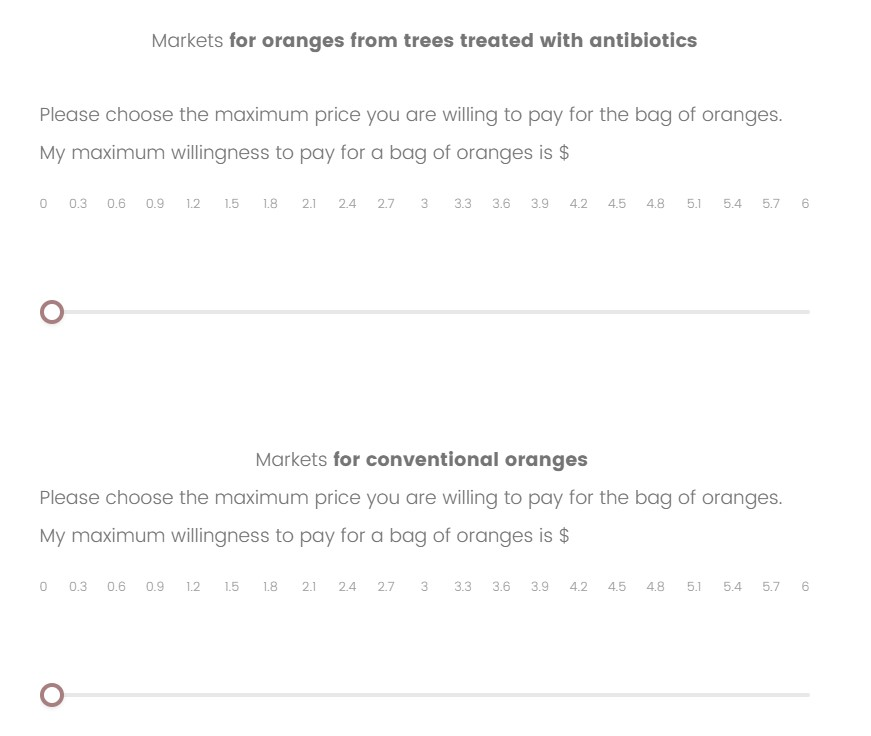
\includegraphics[width=0.8\linewidth]{BDM_market.jpg}

\end{figure}

\clearpage

\definecolor{navyblue}{RGB}{0, 0, 128}

\subsubsection*{Instructions (continued)}
Let me give you an example: Assume that you bid \textbf{\$3.00}, and the fixed price is \textcolor{cyan}{\$2.80}, then you win the orange and only pay \textcolor{cyan}{\$2.80}. If, however, your price was lower than the fixed price, then you do not buy the orange.  

You should offer the maximum price you are willing to pay for the orange; there are no advantages to strategic behavior in this task. Your best strategy is to determine your personal value for the orange and offer that price.  

\vspace{0.3cm}

\textbf{Why is it my best strategy to bid the maximum price I’d be willing to pay?}  

If I truly value the orange at \textbf{\$3.00}, however instead of bidding \textcolor{orange}{\$3.00}, I bid \textcolor{orange}{\$2.60}, and the fixed price is \textcolor{cyan}{\$2.80}, then I lose the opportunity to purchase the oranges. However, had I bid my true valuation I would have won and paid only \textcolor{cyan}{\$2.80} for an orange I think is worth \textbf{\$3.00}.  

Now what if I offer more? Let’s say that I truly valued the orange at \textbf{\$3.00} and I bid \textcolor{orange}{\$5.00}, and the fixed price ended up being \textcolor{orange}{\$4.40}. Then I win, I will have to pay \textcolor{cyan}{\$4.40} for an item I value at \textbf{\$3.00}.  

\vspace{0.5cm} 

When you have understood the instructions, please proceed to the next page.  


\clearpage


\subsubsection*{Instructions continued}


\textbf{Example 1}: If the card you own can be redeemed for a bonus of \$6.00, you bid \$3.00 and the fixed price is \$2.40, you have a higher bid than the fixed price. You buy the item, and you pay the fixed price (\$2.40), plus your balance is (\$6.00 - \$2.40 = \$3.60) and you get the product which will be shipped to your specified mailing address using priority shipping.
\vspace{0.5cm}


\textbf{Example 2}: If the card you own can be redeemed for a bonus of \$6.00, your bid is \$3.00 and the fixed price is \$4.00, you have a bid lower than the fixed price. You do not buy the item, and you receive your bonus of \$6.00.

\vspace{0.5cm}

When you have understood the instructions, please proceed to the next page.
\clearpage


\subsubsection*{Comprehension test}
Note: All following questions will provide simple explanations if the subject indicates or types the wrong answer(correct answer is in bold).

\vspace{0.5cm}

True or False? The fixed price will be a known number to me before I make a decision.  

• True  \par
\textbf{• False}\par  

\vspace{0.5cm}


\vspace{0.5cm}



True or False? My best strategy is to bid the maximum I'd be willing to pay.  

\textbf{• True}  \par
• False 

\vspace{0.5cm}

If I value both oranges at \$5.00:

\textbf{a) Although the value of my card is less than \$10.00, I can bid \$5.00 in each market. However, only one of these bids will be binding.}  

b) I can only bid in one market since the value of my card is less than \$10.00.  

\vspace{0.5cm}

If the card you own could be redeemed for a bonus of \$6.00, your bid was \$4.00 and the fixed price was \$2.4, what would have been your final outcome?  

\textbf{a) I pay \$2.40 for the orange, so my balance is \$6 - \$2.40 = \$3.60 } 

b) The value of my card is \$6.00, since I cannot buy the orange  

c) I pay \$4.00 for the orange, so my balance is \$6.00 - \$4.00 = \$2.00  

\vspace{0.5cm}

If the card you own could be redeemed for a bonus of \$6.00, your bid is \$3.40 and the fixed price is \$4.00, what would be your final outcome?  

d) I pay \$4.00 for the orange, so my balance is \$6.00 - \$4.00 = \$2.00  

\textbf{e) The value of my card is \$6.00, since I cannot buy the orange } 

f) I pay \$3.4 for the orange, so my balance is \$6.00 - \$3.40 = \$2.60  

\vspace{0.5cm}

\subsubsection*{\textbf{Instructions (continued)}}

You have successfully completed the comprehension test, and you will now begin Task 1.\par

\vspace{0.5cm}
 Please click next when you are ready to proceed.

Now, we will go to the main tasks. 

\textbf{Please remember this decision is hypothetical and you will not earn money or a bag of oranges.}

\clearpage

\subsubsection*{\centering \textbf{Round 1 \& 2}}

\begin{figure}[H]
    \centering
    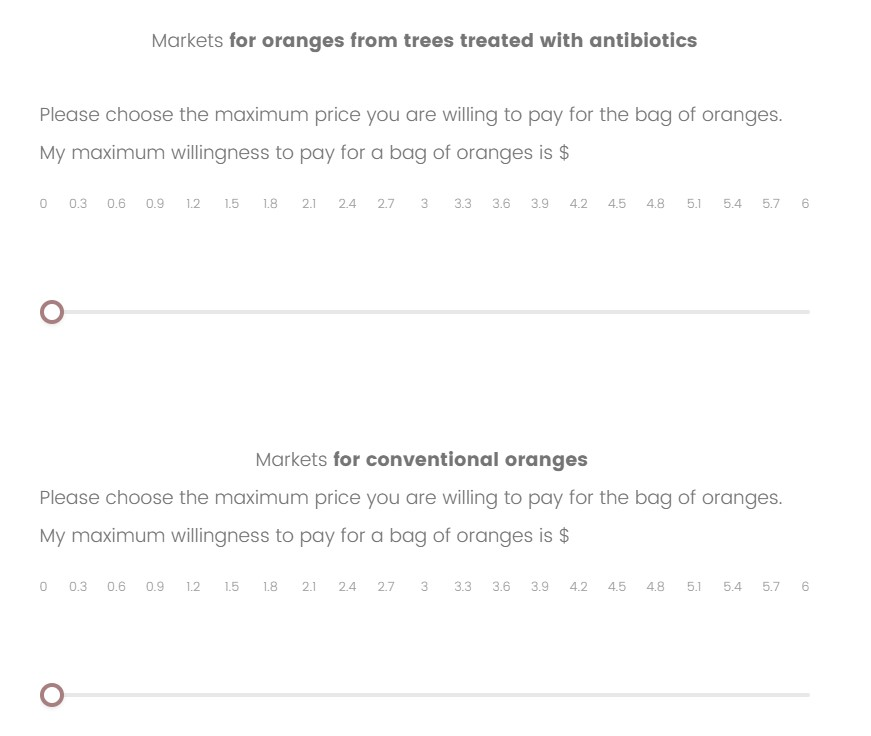
\includegraphics[width=0.8\linewidth]{BDM_market.jpg}
    \caption{}
    \label{fig:BDM_market}
\end{figure}

\clearpage

\subsubsection*{\textbf{Instructions (continued)}}
On the next page, you will see a video. \textbf{Please ensure your speakers or headphones are connected and the volume is set properly.} Next you will see a video that provides information about a disease Watch the video carefully in a quiet, distraction-free environment, as it is essential for the study.
\vspace{0.5cm}
Click on the video to watch it.

\href{https://www.youtube.com/watch?v=_AqMBjB0ChM}{video}
\clearpage


 \subsubsection*{\centering Round 3}


\begin{figure}[H]
    \centering
    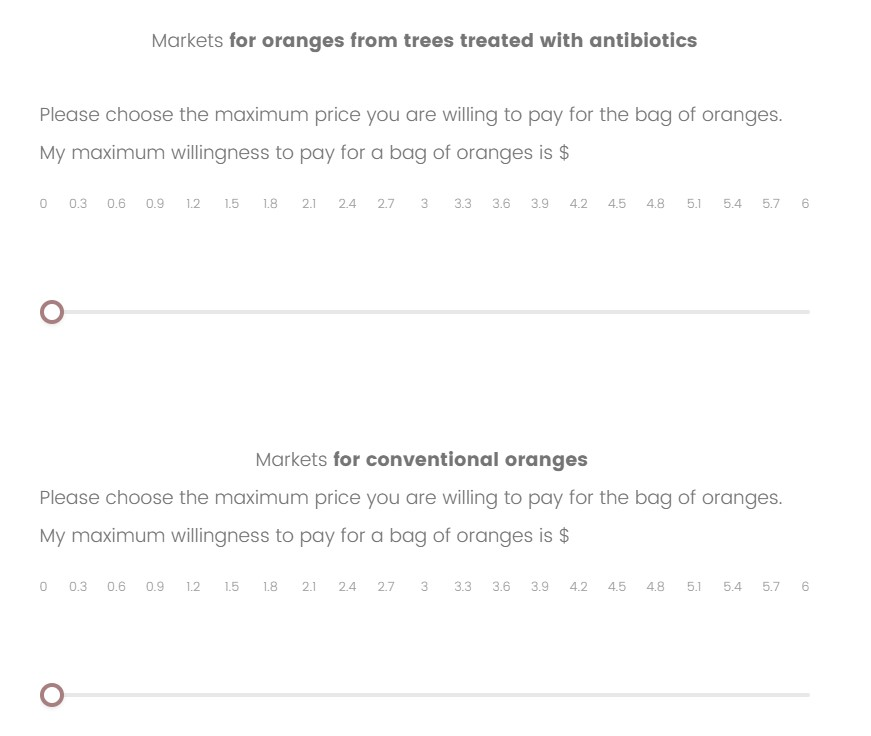
\includegraphics[width=\linewidth]{BDM_market.jpg}
    \caption{}
    \label{fig:BDM_market}
\end{figure}

\clearpage



\subsection{BDM Real}


\subsubsection*{\textbf{Instructions (continued)}}


For this study you will receive a fixed fee of \$2 and you can earn additional compensation in cash and/or citrus products based on your decisions and chance, so please pay attention to the instructions.
 
You will complete 3 Tasks that involve real money, so please pay attention to the instructions. There is a 10\% chance that your decisions will be selected for payment. After completing the 3 tasks, the computer will draw a random number between 1 and 10. If the random number is equal to 1, you will receive the payoff as described below. However, if the random number is between 2 and 10, your decision will not yield additional earnings, and you will receive just the \$2. If you are selected for payment, one of the three tasks will be randomly selected to be added to your compensation.

 Since there is a chance that your decision will end up affecting your earnings, it is in your best interest to respond carefully to each task. If your compensation includes a food product (oranges), the product will be shipped to your specified address *free of charge* via priority mail as long as you provide us with a valid mailing address. You will receive more details about this procedure below.

\clearpage

\subsubsection*{\textbf{Instructions (continued)}}

In this study, you will complete 3 Tasks and a survey.
For each task, you will be endowed with a card with a value of \$6.00. You can use the funds in the card to purchase a bag of oranges (3.2 lbs – approximately 6-8 oranges) in two distinct markets. Any remaining funds in the card that you don’t spend on the oranges will be added to your earnings on top of your \$2.00 participation fee if you are selected for payment.



In one market, the oranges are from trees treated with antibiotics by injection to the *tree’s trunks* (not directly in the orange fruits) to prevent yield and fruit quality losses caused by a disease called citrus greening. The other market is conventional oranges, not from trees treated with antibiotics, but using a combination of pesticides and cultural practices.


You can use the funds in your card to bid on one of the markets or both. Your bid will be compared to an unrelated fixed price that is equally likely to be a number between $0.00 and $6.00. If your bid is higher than the fixed price, you will purchase the item. But here is the interesting part, in this case, you do not pay the price you offer, instead you pay the fixed offer. If your bid is lower than the fixed price, you do not buy the orange and you do not pay anything. 

 

\textbf{Please remember this decision is real and you may earn money or any bag of oranges.}

 

 \clearpage

\subsubsection*{\textbf{Instructions (continued)}}

From that point, the instructions are the same as hypothetical, with a different reminder as shown below;

 Now, we will go to the main tasks.


\textbf{Please remember this decision is real and you may earn money or any bag of oranges.}

 \clearpage

 \subsection{GSO Hypothetical}
 \subsubsection*{\textbf{Instructions (continued)}}

For this study, we will explore your preferences for oranges. You will only receive a participation fee of \$2.00. In the next screen you will be presented with a hypothetical scenario. Note that the scenario is hypothetical, but we ask you to make your decisions as if you were in a real market using real money. Although we will describe the rules of the procedure shortly as if it actually involves money, you will not actually have to pay anything, and we will not ship any products to you. However, we do want you to treat it as if it was real. That is, although you will not receive a bag of oranges and you will not actually have to pay anything, we still want you to formulate your bid thinking what you would do if you had to do it for real. You will receive more details about this procedure below.


\clearpage

\subsubsection*{\textbf{Instructions (continued)}}

In this study, you will complete 3 Tasks and a survey.

For each task, you will be endowed with a card with a value of \$6.00. You can use the funds in the card to purchase a bag of oranges (3.2 lbs – approximately 6-8 oranges) in two distinct markets. Any remaining funds in the card that you don’t spend on the oranges will be added to your earnings on top of your \$2.00 participation fee if you are selected for payment.

In one market, the oranges are treated with antibiotics by injection to the *tree’s trunks* (not directly in the orange fruits) to prevent yield and fruit quality losses caused by a disease called citrus greening. The other market is conventional oranges, not treated with antibiotics, but using a combination of pesticides and cultural practices.

You can use the funds in your card to purchase from one of the markets or both.

 
\textbf{Please remember this decision is hypothetical and you will not earn money or any bag of oranges.}

\clearpage

\subsubsection*{\textbf{Instructions (continued)}}

 In each market, offer prices will be displayed on the screen, and you will make choices over several periods. For every period, you can click “Try to Buy” if you are willing to buy the bag of oranges at the corresponding offer price or click “Not Buy” if you are not willing to buy at that offer price.
The computer has already randomly chosen the \textbf{market price} at which it will accept to sell the bag of oranges to you. That price is drawn between \$0.00 and \$6.00 and is equally likely.

In the first period, the offer price starts at \textcolor{orange}{\$0.00 }and will increase by \$0.20 after every period. The task ends when the price on the screen increases to the \textbf{market price} that the computer chose to sell the bag of oranges.
At every other price, whether you choose “Try to Buy” or “Not Buy”, you will go to the next period and again choose between “Try to Buy” or “Not Buy”.
The task will continue until the offer price reaches the market price the computer chose to try to sell the bag of oranges to you. At that price:

\begin{enumerate}
    \item If you choose “Try to Buy”, you receive the market price, and task ends.
    \item If you choose “Not Buy” you will not be able to buy the bag of oranges and task ends.
\end{enumerate}


For example, let’s say you are in Period 1, when the offer price is \$0.00. If the computer tries to sell you the bag of oranges at that price, and you click “Try to Buy”, you will get the bag of oranges at the current price \$0.00. If instead you clicked “Not Buy”, you will not be able to buy the bag of oranges. However, if the computer does not try to sell you the bag of oranges at that price, you will go to the next period.

\clearpage



\subsubsection*{\textbf{Instructions (continued)}}


Here is a practice screen to familiarize yourself with the buttons or with the way you choose to buy or not buy. Your responses here will not count toward the main study.
Please keep making choices until the buttons turn red, that is when then the market is over.

\begin{figure}[H]
    \centering
    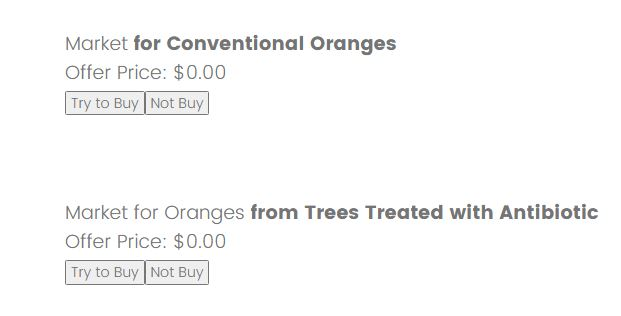
\includegraphics[width=0.8\linewidth]{GSO.JPG}
    
    \label{fig:GSO}
\end{figure}

\clearpage


\subsubsection*{\textbf{Instructions (continued)}}

\textbf{Example 1}

Suppose the maximum amount \textbf{Person X} is willing to pay for the bag of oranges is \textbf{\$3.00}. The first offer price starts at \textcolor{orange}{\$0.00}. Since Person X is willing to purchase the bag of oranges for \textcolor{orange}{\$0.00} (because Person X is willing to pay up to \$3.00), then He/ She would click “Try to Buy” at that offer price.

Suppose the randomly drawn \textbf{market price} from \$0.00 to \$6 is \$2.00 (you will not be able to see it), since the offer price is lower than the market price, Person X would not be able to buy the bag of oranges when selecting “Try to Buy”. He/ She will proceed to the next period where offer price will be \textcolor{orange}{\$0.20}.
Since Person X is willing to purchase the bag of oranges at \$0.20, He/ She would select “Try to Buy”. Once again, the offer price will be compared to the market price. Since the randomly drawn market price in our example was \$2.00, Person X would not buy the bag oranges and He/ She will proceed to the next offer price of \textcolor{orange}{\$0.40}.


This process will continue until the offer price is \textcolor{orange}{\$2.00}. When the offer price is \textcolor{orange}{\$2.00}, Person X chooses “try to buy” and since the market price is \textcolor{cyan}{\$2.00} a transaction will occur at that time. Note that Person X maximum willingness to pay for the bag of oranges was \textbf{\$3.00}, but the market price randomly generated by the computer was \textcolor{cyan}{\$2.00}. So, if selected for payment, Person X would purchase the bag of oranges and receive them via priority shipping to their designated mailing address and the remaining \$4.00 on their card will be added to their compensation.



Please proceed to the next page for another example.
\clearpage

\subsubsection*{\textbf{Instructions (continued)}}

Example 2

Suppose the maximum amount \textbf{Person X} is willing to pay for the bag of oranges is \textbf{\$3.00}. The first offer price starts at \textcolor{orange}{\$0.00}. Since Person X is willing to purchase the bag of oranges for \textcolor{orange}{\$0.00} (because Person X is willing to pay up to \$3.00), then He/ She would click “Try to Buy” at that offer price.

Suppose the randomly drawn market price from \$0.00 to \$6.00 is \textcolor{cyan}{\$4.00} (you will not be able to see it), since the offer price is lower than the market price, Person X would not be able to buy the bag of oranges when selecting “Try to Buy”. He/ She will proceed to the next period where offer price will be \textcolor{orange}{\$0.20}.

Since Person X is willing to purchase the bag of oranges at \textcolor{orange}{\$0.20}, He/ She would select “Try to Buy”. Once again, the offer price will be compared to the market price. Since the randomly drawn market price in our example was \textcolor{cyan}{\$4.00}, Person X would not buy the bag oranges, and He/ She will proceed to the next offer price of \textcolor{orange}{\$0.40}.


This process will continue until the offer price is \textcolor{orange}{\$3.00}.  However, in the next round, the offer price will be \textcolor{orange}{\$3.20}. When the offer price is \textcolor{orange}{\$3.20}, Person X would click “Not buy”. When clicking “Not buy”, she will go to the next round and will continue to click “Not Buy” until task ends and will not be able to buy the bag of oranges. In this example, task ends when the offer price reaches \textcolor{cyan}{\$4.00}. Person X will click “Not Buy” at this price and will not be able to buy the bag of oranges.
\vspace{0.5cm}

When you have understood the instructions, please proceed to the next page.
\clearpage

\subsubsection*{Comprehension test}

Select which statement below is the most correct

\begin{itemize}
    \item The price increases by \$0.20 in each subsequent period 
    \item The value of your card does not change
    \item \textbf{Both answers are true}
\end{itemize}

\vspace{0.5cm}

What will happen to your reward if you try to buy when the fixed price is \$4.40, and the computer accepts your price?

\begin{itemize}
    \item I will get \$6, which is the value of my card
    \item \textbf{I will pay the oranges at \$4.40, plus get my balance of \$6.00-4.40=\$1.60}
    \item It is random
\end{itemize}

\vspace{0.5cm}


If the price of oranges in both markets is \$5.00 at a given period, can I try to buy both oranges in both markets?

\begin{itemize}
    \item No, you can’t because your card is worth \$6, it exceeds your endowment.
    \item \textbf{Yes, you can, however if the computer accepts both prices, only one decision will be randomly binding for realization.}
\end{itemize}

\vspace{0.5cm}

If Person' X maximum willingness to pay for the orange is \$3.00, S/He would switch from "Try to Buy" to "Not Buy" at \$3.20.

\begin{itemize}
    \item \textbf{Then Person X will continue to click "Not Buy" until the market ends}
    
    \item Person X should try to switch back and forth to "Try to Buy" and "Not Buy"
    \item None of these answers is correct
\end{itemize}

\clearpage



\subsubsection*{Comprehension test (continued)}

You have successfully completed the comprehension test, and you will now begin Task 1.

 Please click next when you are ready to proceed.

 Now, we will go to the main tasks. 
 
 \textbf{Please remember this decision is hypothetical and you will not earn money or any bag of oranges.}


\clearpage

 \subsubsection*{Round 1\& 2}


 \begin{figure}[H]
    \centering
    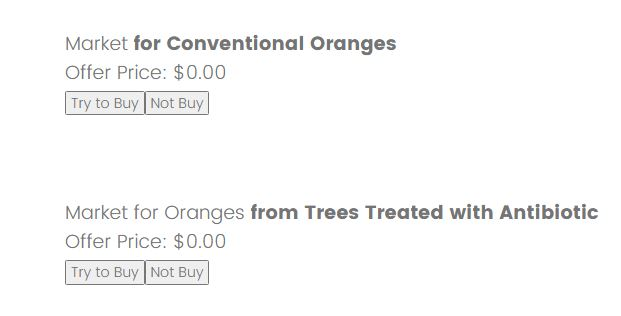
\includegraphics[width=0.8\linewidth]{GSO.JPG}
    
    \label{fig:GSO}
\end{figure}

 \vspace{0.5cm}


On the next page, you will see a video. \textbf{Please ensure your speakers or headphones are connected and the volume is set properly.} Next you will see a video that provides information about a disease Watch the video carefully in a quiet, distraction-free environment, as it is essential for the study.
\vspace{0.5cm}
Click on the video to watch it.

\href{https://www.youtube.com/watch?v=_AqMBjB0ChM}{video}
\clearpage


 \subsubsection*{Round 3}



\begin{figure}[H]
    \centering
    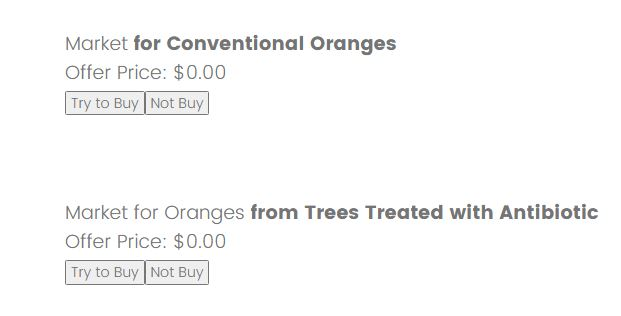
\includegraphics[width=\linewidth]{GSO.JPG}
    \caption{}
    \label{fig:Appendix_GSO_game}
\end{figure}
 

\clearpage



\subsection{GSO Real}

\subsubsection*{Instructions}

For this study you will receive a fixed fee of \$2.00 and you can earn additional compensation in cash and/or citrus products based on your decisions and chance, so please pay attention to the instructions.
 
You will complete 3 Tasks that involve real money, so please pay attention to the instructions. There is a 10\% chance that your decisions will be selected for payment. After completing the 3 tasks, the computer will draw a random number between 1 and 10. If the random number is equal to 1, you will receive the payoff as described below.
However, if the random number is between 2 and 10, your decision will not yield additional earnings, and you will receive just the \$2.00. If you are selected for payment, one of the three tasks will be randomly selected to be added to your compensation.

\textbf{Since there is a chance that your decision will end up affecting your earnings, it is in your best interest to respond carefully to each task}. If your compensation includes a food product (oranges), the product \textbf{will be shipped to your specified address *free of charge* via priority mail} as long as you provide us with a valid mailing address. You will receive more details about this procedure below.


\clearpage

\subsubsection*{Instructions (continued)}

In this study, you will complete 3 Tasks and a survey.

For each task, you will be endowed with a card with a value of \$6.00. You can use the funds in the card to purchase a bag of oranges (3.2 lbs – approximately 6-8 oranges) in two distinct markets. Any remaining funds in the card that you don’t spend on the oranges will be added to your earnings on top of your \$2.00 participation fee if you are selected for payment.

In one market, the oranges are from trees treated with antibiotics by injection to the *tree’s trunks* (not directly in the orange fruits) to prevent yield and fruit quality losses caused by a disease called citrus greening. The other market is conventional oranges, not from trees treated with antibiotics, but using a combination of pesticides and cultural practices.

You can use the funds in your card to purchase from one of the markets or both.

\textbf{ Please remember this decision is real and you may earn money or any bag of oranges.}

\clearpage

\subsubsection*{Instructions (continued)}

 From that point, the instructions are the same as hypothetical, with a different reminder as shown below;

 Now, we will go to the main tasks.
\vspace{0.5cm}

\textbf{Please remember this decision is real and you may earn money or any bag of oranges.}


 \clearpage

\section{Background on citrus greening}
\label{AppedixOrange}
 The United States, which was once the world leader in citrus production, producing 50\% of the world's citrus in 1970, has experienced a decrease in its global share to 25\% in 2000, then to 5\% in 2023 \citep{munch_us_2023} . As a result of this staggering decline in domestic production, the country relies more on imports from countries such as Mexico and Chile. The recent decline in citrus production over the past 15 years in the US is mainly a result of a bacterial disease known as "Huanglongbing" (HLB) or citrus greening. This disease was first discovered in Florida in 2005, it accounts; for the infection of 80\% of citrus plants in Florida \citep{li2020citrus} and increases  production cost of farmers \citep{roka2009citrus} . This disease, caused by the bacteria "Liberibacter asiaticus", results in chlorosis of the foliage, reduction of absorption of nutrients and yield, and death of citrus trees within 3 years \citep{bove_huanglongbing_2006}. The citrus greening also affects the marketability of the citrus by distorting its size, visual feature, ripening (partial or not at all), and flavor \citep{farnsworth_potential_2024}. Orange juice made from infected citrus fruit has a higher concentration of limonin and nomilin leading to a sour taste of citrus juice \citep{paula2018active}. 

Previously, to address HLB, systematic tree removal was recommended to combat HLB. However, this approach was not sustainable for multiple reasons. First, symptomatic citrus trees could still produce some marketable fruit, making immediate tree removal financially cumbersome for farmers. Second, replacing an infected tree with a new one incurs high costs for farmers, as it takes several years before new trees begin to bear fruit.  Finally, the effect of tree removal is undermined by the external cost. If some farmers decide not to remove infected trees, the disease contributes to spreading, negating the effort of others \citep{farnsworth_potential_2024}. Recently, the administration of antibiotics through trunk injections has been investigated and found to be a promising method to control HLB \citep{li_precision_2022}. \citet{archer_trunk_2023} corroborates this discovery by showing that the administration of oxytetracyclin through injection into the trunk of orange trees results in a decrease in fruit loss before harvest, as well as an improvement in fruit output, size, and juice quality.

Antibiotics administration has been applied for decades in cattle. However, according to \citet{hosain_antimicrobial_2021}, it has drawbacks on human health; it accounts for 80\% of antimicrobial resistance (AMR) in USA annually, and AMR affects 2.8 million people, causing more than 35.000 deaths \citep{cdc2019antibiotic}.  The use of antibiotics can effectively help to manage the dissemination of HLB, thus protecting citrus trees. Consequently, this can be advantageous to citrus farmers and all other stakeholders involved in the citrus industry at the state level in Florida. Antibiotics can help decrease Florida's reliance on imported citrus, thus preventing the probable extinction of citrus at the state level. This is undesirable for those who enjoy Florida citrus fruits and juice, as well as those who prefer locally sourced products. Ultimately, it can help preserve the superior taste of juice, preventing the occurrence of a bitter flavor that may arise from citrus fruits obtained from infected trees. The use of antibiotics also comes with some challenges. First, it may cause health hazards (AMR) if relevant policy is not reinforced on dosage and injection timing. Second, it may leave  residues in wastewater that could lead to soil pollution. In light of this dilemma, it directs our attention to determining how consumers will respond to the use of antibiotics in the production of citrus fruit since the success of such techniques depends on the acceptance of consumers, which also depends on the way information is communicated. Although the use of antibiotics in livestock has been extensively studied, it is unfortunate that the literature is silent about consumers’ preference for foods treated with antibiotics; hence, we propose filling this gap.

\clearpage










\section{Tables for main results}

\begin{table}[htbp]
\centering
\footnotesize
\caption{Standardized Differences comparing participants included vs excluded in the study}
\label{tab:Incomplete}
\begin{threeparttable}
\begin{tabular}{llccc}
\toprule
\textbf{Variable} & \textbf{Category} & \textbf{Include} & \textbf{Exclude} & \textbf{Std. Diff} \\
\midrule
\multirow{2}{*}{Ethnicity} & Non-White & 413 (34.90\%) & 345 (31.10\%) & 0.08 \\
                           & White     & 771 (65.10\%) & 766 (68.90\%) & \\
\midrule
\multirow{3}{*}{Income Category} & Low income    & 537 (46.3\%) & 535 (50.90\%) & 0.14 \\
                                 & Middle income & 519 (44.70\%) & 397 (37.80\%) & \\
                                 & High income   & 104 (9\%)  & 119 (11.30\%) & \\
\midrule
\multirow{4}{*}{Region} & Northeast & 200 (16.90\%) & 196 (17.70\%) & 0.07 \\
                        & Midwest   & 265 (22.40\%) & 259 (23.40\%) & \\
                        & South     & 464 (39.30\%) & 397 (35.80\%) & \\
                        & West      & 252 (21.30\%) & 257 (23.20\%) & \\
\midrule
\multirow{2}{*}{Gender} & Male   & 573 (49.10\%) & 523 (48.20\%) & 0.02 \\
                        & Female & 593 (50.90\%) & 562 (51.80\%) & \\
\midrule
\multirow{2}{*}{Education} & No Bachelor & 751 (63.40\%) & 701 (63.10\%) & 0.007 \\
                           & Bachelor    &  433   (36.60\%)        &   410 (36.90\%)          &  \\
\midrule
\multirow{2}{*}{Children} & Children     & 405 (35\%) & 207 (19.80\%) & 0.34 \\
                          & No Children  & 753 (65\%) & 839 (80.20\%) & \\
\midrule
\multirow{2}{*}{Marital Status} & Married     & 419 (35.40\%) & 365 (32.90\%) & 0.05 \\
                                & Not Married &   765 (64.60\%)          &    746 (67.10\%)         & \\
\midrule
Age  & & 46 (16.53) & 53.32 (17.96) & -0.424 \\
\bottomrule
\end{tabular}
\begin{tablenotes}

\item \textit{Notes: }Standardized differences are calculated between those included and excluded in the study. Number not in parentheses represent number of participants, those in parentheses represent proportions for categorical variables and standard deviations for continuous ones.
\end{tablenotes}
\end{threeparttable}
\end{table}

\clearpage


    \begin{table}[htbp!]
\centering
\caption{Standardized Differences Across Variables}
\label{tab:Appendix_std_diff_table}
\resizebox{\textwidth}{!}{%
\begin{tabular}{lcccccc}
\hl& \multicolumn{3}{c}{\textbf{GSO Real vs.}} & \multicolumn{2}{c}{\textbf{BDM Real vs.}} & \textbf{GSO Hypo vs.} \\
\cmidrule(lr){2-4} \cmidrule(lr){5-6} \cmidrule(lr){7-7}
\textbf{Variable}        & \textbf{BDM Real} & \textbf{GSO Hypo} & \textbf{BDM Hypo} & \textbf{GSO Hypo} & \textbf{BDM Hypo} & \textbf{BDM Hypo} \\
\hline

Hispanic        & 0.0884        & 0.0114        & 0.0630        & 0.0770        & 0.0254        & 0.0516 \\
Income category        & 0.1704        & 0.0462        & 0.1440        & 0.1498        & 0.0431        & 0.1153 \\
Region  & 0.1326        & 0.1861        & 0.1918        & 0.1064        & 0.0779        & 0.0850 \\
Gender  & 0.0834        & 0.0178        & 0.0228        & 0.0927        & 0.0627        & 0.0379 \\
Education       & 0.2267        & 0.1748        & 0.1342        & 0.0514        & 0.0919        & 0.0404 \\
children        & 0.0584        & 0.0128        & 0.0869        & 0.0456        & 0.0284        & 0.0740 \\
Marital status  & 0.0952        & 0.0322        & 0.0437        & 0.1274        & 0.0514        & 0.0759 \\
Age     & -0.0160       & 0.0753        & -0.0557       & 0.0883        & -0.0380       & -0.1285 \\

\hline \hline
\end{tabular}}
\begin{tablenotes}
\item Notes: GSO stands for the Game Structure Obvious mechanism treatment; BDM stands for the Becker-DeGroot-Marschak mechanism treatment; Real and Hypothetical stand for the real and hypothetical incentives treatments, respectively.
\end{tablenotes}
\end{table}
  
 
\clearpage


        % Right column for the second table

            \begin{table}[htbp]
                \centering
                \caption{Descriptive Statistics by Treatment 
                (excluding excluding MS (R1: 14.2\%, R2, 9.6\%, R3: 3.6\%)
)}
                \label{tab:Appendix_descrip_2}
                \resizebox{1\textwidth}{!}{%
                \begin{tabular}{lccc}
                \hline \hline
                \textbf{Treatment}    & \textbf{N (including MSB)}       & \textbf{Mean (USD)}  & \textbf{Standard Deviation} \\
                \hline
                GSO Real           & 288                        & 3.50       & 1.20                  \\
                BDM Real            & 313                        & 3.48       & 1.36                \\
                GSO Hypothetical     & 295                     & 3.63      & 1.16                   \\
                BDM Hypothetical      & 320                  & 3.44       & 1.30                    \\
                \midrule
                \textbf{Total}         & \textbf{1,216}              & \textbf{3.48} & \textbf{1.26}         \\
                \hline\hline
              
                \end{tabular}}
\begin{tablenotes}    
            \item Notes: GSO stands for the Game Structure Obvious mechanism treatment; BDM stands for the Becker-DeGroot-Marschak mechanism treatment; Real and Hypo stand for the real and hypothetical incentives treatments, respectively.
        \end{tablenotes}
            \end{table}
       
     
\clearpage
  











 \begin{table}[H]
                \centering
                \caption{Interval Model of Consumer WTP for Oranges (Baseline: BDM Real)}
                \label{tab:interval_regression}
                \resizebox{\textwidth}{!}{% Scale table to fit the column width
    \begin{tabular}{l*{4}{cc}}
    \hline \hline
            &\multicolumn{2}{c}{WTP}    &\multicolumn{2}{c}{WTP (control 1)}    &\multicolumn{2}{c}{WTP (control 2)}    &\multicolumn{2}{c}{WTP (control 3)}    \\
    \hline        
Constant    &       3.476\sym{***}&     (0.050)&       3.476\sym{***}&     (0.050)&       3.210\sym{***}&     (0.138)&       3.197\sym{***}&     (0.138)\\
GSO         &       0.042         &     (0.080)&                     &            &       0.027         &     (0.080)&                     &            \\
Hypothetical&      -0.016         &     (0.070)&      -0.016         &     (0.070)&      -0.030         &     (0.070)&      -0.030         &     (0.070)\\
GSOXHypothetical&       0.258\sym{**} &     (0.110)&                     &            &       0.311\sym{***}&     (0.113)&                     &            \\
GSOnoMSB    &                     &            &       0.029         &     (0.082)&                     &            &       0.011         &     (0.082)\\
GSOnoMSBXHypothetical&                     &            &       0.228\sym{**} &     (0.113)&                     &            &       0.280\sym{**} &     (0.116)\\
GSOMSB      &                     &            &       0.228         &     (0.211)&                     &            &       0.252         &     (0.215)\\
GSOMSBXHypothetical&                     &            &       0.517\sym{**} &     (0.261)&                     &            &       0.571\sym{**} &     (0.266)\\
Round2      &                     &            &                     &            &       0.049\sym{*}  &     (0.027)&       0.052\sym{*}  &     (0.027)\\
Round3      &                     &            &                     &            &       0.092\sym{***}&     (0.030)&       0.102\sym{***}&     (0.030)\\
White       &                     &            &                     &            &      -0.045         &     (0.064)&      -0.043         &     (0.064)\\
Middle Income&                     &            &                     &            &      -0.079         &     (0.064)&      -0.081         &     (0.064)\\
High Income &                     &            &                     &            &      -0.015         &     (0.115)&      -0.013         &     (0.115)\\
Midwest     &                     &            &                     &            &      -0.176\sym{**} &     (0.087)&      -0.181\sym{**} &     (0.086)\\
South       &                     &            &                     &            &      -0.079         &     (0.078)&      -0.080         &     (0.078)\\
West        &                     &            &                     &            &      -0.112         &     (0.085)&      -0.118         &     (0.085)\\
Female      &                     &            &                     &            &       0.032         &     (0.054)&       0.037         &     (0.054)\\
Bachelor    &                     &            &                     &            &      -0.048         &     (0.061)&      -0.046         &     (0.060)\\
No Children &                     &            &                     &            &       0.019         &     (0.068)&       0.024         &     (0.068)\\
Married     &                     &            &                     &            &      -0.061         &     (0.061)&      -0.063         &     (0.061)\\
Age         &                     &            &                     &            &       0.009\sym{***}&     (0.002)&       0.009\sym{***}&     (0.002)\\
\hline
$\sigma_u $    &       1.091\sym{***}&     (0.019)&       1.088\sym{***}&     (0.019)&       1.080\sym{***}&     (0.019)&       1.077\sym{***}&     (0.019)\\
$\sigma_e $     &       0.846\sym{***}&     (0.020)&       0.846\sym{***}&     (0.020)&       0.845\sym{***}&     (0.019)&       0.844\sym{***}&     (0.019)\\
\hline
\(n\) (observations)      &        7104         &            &        7104         &            &        6828         &            &        6828         &            \\

\(N \) (subjects)      &        1184         &            &        1184         &            &        1138         &            &        1138         &            \\
\hline \hline
\end{tabular}
}




\begin{tablenotes}
          \footnotesize
           \item \textit{Notes:} Bootstrap Standard errors (1000 times) in parentheses. * p$<$0.1, ** p$<$0.05, *** p$<$0.01. $\sigma_u$ and $\sigma_e$ denote the standard deviations of the random intercept and residual error, respectively. GSO stands for the Game Structure Obvious mechanism treatment; BDM stands for the Becker-DeGroot-Marschak mechanism treatment; Real and Hypo stand for the real and hypothetical incentives treatments, respectively. $\times$: interaction GSOnoMSB: A dummy variable for being GSO and no MS. GSOMSB: A dummy variable for being GSO and with MS.
             Baseline: BDM Real represents the baseline treatment group of the regression analysis.
        \end{tablenotes}
            \end{table}

\clearpage







\begin{table}[H]
        \centering
      \caption{Comparison of Willingness to Pay by Instruction Comprehension Scores (demean Quiz) }
        \label{tab:MSB_interval_regression_Score_overall}
       \resizebox{0.7\textwidth}{!}{% Scale table to fit the column width
      \begin{tabular}{l*{1}{cc}}
      \hline \hline
            &\multicolumn{2}{c}{WTP (BDM Real: baseline)}    \\
            \hline
Constant    &       3.096\sym{***}&     (0.140)\\
GSO         &       0.085         &     (0.083)\\
Hypothetical&       0.125         &     (0.078)\\
GSO$\times$Hypothetical&       0.162         &     (0.118)\\
Testscore  &       0.052\sym{**} &     (0.023)\\
GSO$\times$Testscore&      -0.157\sym{***}&     (0.038)\\
Hypothetical$\times$Testscore&       0.017         &     (0.036)\\
GSO$\times$Hypothetical$\times$Testscore&       0.006         &     (0.055)\\
Round2      &       0.049\sym{*}  &     (0.027)\\
Round3      &       0.092\sym{***}&     (0.030)\\
White       &      -0.043         &     (0.065)\\
Middle Income&      -0.056         &     (0.064)\\
High Income &       0.005         &     (0.115)\\
Midwest     &      -0.154\sym{*}  &     (0.086)\\
South       &      -0.075         &     (0.077)\\
West        &      -0.103         &     (0.085)\\
Female      &       0.033         &     (0.053)\\
Bachelor    &      -0.040         &     (0.061)\\
No Children &       0.030         &     (0.068)\\
Married     &      -0.039         &     (0.061)\\
Age         &       0.009\sym{***}&     (0.002)\\
\hline
$\sigma_u $    &       1.069\sym{***}&     (0.020)\\
$\sigma_e $     &       0.845\sym{***}&     (0.019)\\
\hline
\(n\) (observations)      &        6828         &            \\
\(N\) (subjects)       &        1138         &            \\
\hline \hline
\end{tabular}
}

\begin{tablenotes}
            \footnotesize
            \item \textit{Note:} Bootstrap Standard errors (1000 times) in parentheses.  $\sigma_u$ and $\sigma_e$ denote the standard deviations of the random intercept and residual error, respectively. GSO stands for the Game Structure Obvious mechanism treatment; BDM stands for the Becker-DeGroot-Marschak mechanism treatment; Real and Hypo stand for the real and hypothetical incentives treatments, respectively. $\times$: Interaction.
           \item Baseline: BDM Real. represents the baseline treatment group for the right hand-side. * p$<$0.1, ** p$<$0.05, *** p$<$0.01.
        \end{tablenotes}
\end{table}



\clearpage






\begin{table}[H]
        \centering
      \caption{Comparison of Willingness to Pay by Complexity Scores (demean complexity) }
        \label{tab:Complexity}
       \resizebox{0.7\textwidth}{!}{% Scale table to fit the column width
      \begin{tabular}{l*{1}{cc}}
      \hline \hline
            &\multicolumn{2}{c}{WTP (BDM Real: baseline)}    \\
            \hline
Constant    &       3.218\sym{***}&     (0.139)\\
GSO         &       0.029         &     (0.081)\\
Hypothetical&      -0.019         &     (0.072)\\
GSO$\times$Hypothetical&       0.308\sym{***}&     (0.114)\\
Complexityscore  &       0.013         &     (0.048)\\
GSO$\times$Complexityscore&       0.021         &     (0.084)\\
Hypothetical$\times$Complexityscore&      -0.089         &     (0.069)\\
GSO$\times$Hypothetical$\times$Complexityscore&       0.161         &     (0.109)\\
Round2      &       0.049\sym{*}  &     (0.027)\\
Round3      &       0.092\sym{***}&     (0.030)\\
White       &      -0.043         &     (0.065)\\
Middle Income&      -0.083         &     (0.065)\\
High Income &      -0.023         &     (0.115)\\
Midwest     &      -0.179\sym{**} &     (0.087)\\
South       &      -0.085         &     (0.078)\\
West        &      -0.114         &     (0.085)\\
Female      &       0.027         &     (0.054)\\
Bachelor    &      -0.042         &     (0.061)\\
No Children &       0.023         &     (0.068)\\
Married     &      -0.066         &     (0.061)\\
Age         &       0.009\sym{***}&     (0.002)\\
\hline
$\sigma_u $    &       1.078\sym{***}&     (0.019)\\
$\sigma_e$     &       0.845\sym{***}&     (0.019)\\

\hline
\(n\) (observations)      &        6828         &            \\
\(N\) (subjects)       &        1138         &            \\
\hline \hline
\end{tabular}
}

\begin{tablenotes}
            \footnotesize
             \item Notes: Bootstrap Standard errors (1000 times) in parentheses. $\sigma_u$ and $\sigma_e$ denote the standard deviations of the random intercept and residual error, respectively. GSO stands for the Game Structure Obvious mechanism treatment; BDM stands for the Becker-DeGroot-Marschak mechanism treatment; Real and Hypo stand for the real and hypothetical incentives treatments, respectively. $\times$: Interaction. Baseline: BDM Real. represents the baseline treatment group for the right hand-side.  * p$<$0.1, ** p$<$0.05, *** p$<$0.01.
        \end{tablenotes}
\end{table}



\clearpage





 \begin{table}[H]
        \centering
        \caption{Comparison of Willingness to Pay (social desirability)}
        \label{tab:interval_regression_socialdesirability_BDM}
        \resizebox{0.8\textwidth}{!}{% Scale table to fit the column width
     \begin{tabular}{l*{1}{cc}}
\hline\hline
            &\multicolumn{2}{c}{WTP (BDM Real: baseline)}    \\
\hline
Constant    &       3.474\sym{***}&     (0.249)\\
GSO         &       0.011         &     (0.147)\\
Hypothetical&       0.146         &     (0.131)\\
GSO$\times$Hypothetical&       0.211         &     (0.203)\\
Information&       0.167\sym{**} &     (0.075)\\
GSO$\times$Information&      -0.026         &     (0.136)\\
Hypothetical$\times$Information&      -0.120         &     (0.109)\\
GSO$\times$Hypothetical$\times$Information&      -0.113         &     (0.195)\\
White       &      -0.224\sym{**} &     (0.113)\\
Middle Income&      -0.121         &     (0.115)\\
High Income &       0.110         &     (0.226)\\
Midwest     &      -0.158         &     (0.170)\\
South       &       0.017         &     (0.154)\\
West        &      -0.200         &     (0.171)\\
Female      &       0.104         &     (0.100)\\
Bachelor    &       0.043         &     (0.108)\\
No Children &       0.164         &     (0.116)\\
Married     &      -0.169         &     (0.114)\\
Age         &       0.006\sym{*}  &     (0.003)\\
$\sigma_u$     &       1.007\sym{***}&     (0.035)\\
$\sigma_e$      &       0.848\sym{***}&     (0.034)\\
\hline
\(n\) (observations)      &        2160         &            \\
\(N\) (subjects)        &        2160         &            \\
\hline\hline
\multicolumn{5}{l}{\footnotesize Standard errors in parentheses. * p$<$0.1, ** p$<$0.05 *** p$<$0.01}\\
\end{tabular}
}

\begin{tablenotes}
            \footnotesize
            \item \textit{Note:} Bootstrap Standard errors (1000 times) in parentheses.  $\sigma_u$ and $\sigma_e$ denote the standard deviations of the random intercept and residual error, respectively. GSO stands for the Game Structure Obvious mechanism treatment; BDM stands for the Becker-DeGroot-Marschak mechanism treatment; Real and Hypo stand for the real and hypothetical incentives treatments, respectively. $\times$: Interaction. Baseline: BDM Real. represents the baseline treatment group. Yes: Represents the sample of participants who mention they would support antibiotics treatment for citrus. * p$<$0.1, ** p$<$0.05, *** p$<$0.01.
        \end{tablenotes}
\end{table}

\clearpage







 \begin{table}[H]
        \centering
        \caption{Comparison of Willingness to Pay by Type of Oranges}
        \label{tab:Orange_socialdesirability_BDM}
        \resizebox{0.8\textwidth}{!}{% Scale table to fit the column width
        \begin{tabular}{l*{1}{cc}}
\hline\hline
            &\multicolumn{2}{c}{WTP (BDM Real: baseline)}    \\
\hline
Constant    &       3.175\sym{***}&     (0.140)\\
GSO         &       0.051         &     (0.089)\\
Hypothetical&      -0.058         &     (0.077)\\
GSO$\times$Hypothetical&       0.374\sym{***}&     (0.124)\\
AntibioticsOranges&       0.069         &     (0.060)\\
GSO$\times$AntibioticsOranges&      -0.048         &     (0.090)\\
Hypothetical$\times$AntibioticsOranges&       0.057         &     (0.081)\\
GSO$\times$Hypothetical$\times$AntibioticsOranges&      -0.129         &     (0.124)\\
Round2      &       0.049\sym{*}  &     (0.027)\\
Round3      &       0.093\sym{***}&     (0.030)\\
White       &      -0.045         &     (0.064)\\
Middle Income&      -0.079         &     (0.064)\\
High Income &      -0.015         &     (0.115)\\
Midwest     &      -0.175\sym{**} &     (0.087)\\
South       &      -0.079         &     (0.078)\\
West        &      -0.112         &     (0.085)\\
Female      &       0.032         &     (0.054)\\
Bachelor    &      -0.047         &     (0.061)\\
No Children &       0.019         &     (0.068)\\
Married     &      -0.062         &     (0.061)\\
Age         &       0.009\sym{***}&     (0.002)\\
$\sigma_u$     &       1.081\sym{***}&     (0.019)\\
$\sigma_e$      &       0.844\sym{***}&     (0.019)\\
\hline
\(N\)       &        6828         &            \\
\hline\hline
\multicolumn{5}{l}{\footnotesize Standard errors in parentheses. * p$<$0.1, ** p$<$0.05 *** p$<$0.01}\\
\end{tabular}
}

\begin{tablenotes}
            \footnotesize
           \item \textit{Note:} Bootstrap Standard errors (1000 times) in parentheses. * p$<$0.1, ** p$<$0.05, *** p$<$0.01.  $\sigma_u$ and $\sigma_e$ denote the standard deviations of the random intercept and residual error, respectively.  GSO stands for the Game Structure Obvious mechanism treatment; BDM stands for the Becker-DeGroot-Marschak mechanism treatment; Real and Hypo stand for the real and hypothetical incentives treatments, respectively. $\times$: Interaction. Baseline: BDM Real. represents the baseline treatment group for the right hand-side. Antibiotics oranges: A dummy variable equal to 1 for oranges from trees treated with antibiotics as compared to conventional oranges.
        \end{tablenotes}
\end{table}







\begin{table}[H]
        \centering
        \caption{Comparison of Willingness to Pay by Round for GSO}
        \label{tab:interval_regression_RounbyRound}
    \resizebox{0.8\textwidth}{!}{%
     \begin{tabular}{l*{1}{cc}}
\hline\hline
            &\multicolumn{2}{c}{WTP (BDM Real: baseline)}    \\
    \hline
    Constant & 3.206\sym{***} & (0.139) \\
    GSO & 0.013 & (0.093) \\
    Hypothetical & -0.045 & (0.079) \\
    GSO$\times$Hypothetical & 0.422\sym{***} & (0.134) \\
    Round2 & 0.075 & (0.048) \\
    Round3 & 0.081 & (0.053) \\
    GSO$\times$Round2 & 0.018 & (0.084) \\
    GSO$\times$Round3 & 0.019 & (0.092) \\
    Hypothetical $\times$ Round2 & -0.032 & (0.067) \\
    Hypothetical$\times$Round3 & 0.076 & (0.075) \\
    GSO$\times$Hypothetical$\times$Round2 & -0.103 & (0.117) \\
    GSO$\times$Hypothetical$\times$Round3 & -0.227\sym{*} & (0.133) \\
    White & -0.045 & (0.064) \\
    Middle Income & -0.079 & (0.064) \\
    High Income & -0.015 & (0.115) \\
    Midwest & -0.175\sym{**} & (0.087) \\
    South & -0.079 & (0.078) \\
    West & -0.112 & (0.085) \\
    Female & 0.032 & (0.054) \\
    Bachelor & -0.047 & (0.061) \\
    No Children & 0.019 & (0.068) \\
    Not Married & -0.063 & (0.061) \\
    Age & 0.009\sym{***} & (0.002) \\
    \hline
    $\sigma_u$ & 1.080\sym{***} & (0.019) \\
   $\sigma_e$ & 0.845\sym{***} & (0.019) \\
    \hline
\(n \) (observations)      &        6828                 \\
\(N \) (subjects)      &        1138           \\
\hline\hline
    
    \end{tabular}
    }



\begin{tablenotes}
            \footnotesize
            \item \textit{Note:} Bootstrap Standard errors (1000 times) in parentheses. $\sigma_u$ and $\sigma_e$ denote the standard deviations of the random intercept and residual error, respectively.Notes: GSO stands for the Game Structure Obvious mechanism treatment; BDM stands for the Becker-DeGroot-Marschak mechanism treatment; Real and Hypo stand for the real and hypothetical incentives treatments, respectively. $\times$: Interaction. GSOMSB: A dummy variable for being GSO and with MS. Baseline: BDM Real. represents the baseline treatment group for the right hand-side. GSO Real represents the Baseline treatment group for the left-hand side. * p$<$0.1, ** p$<$0.05, *** p$<$0.01.
        \end{tablenotes}
\end{table}











\clearpage



\begin{table}[H]
        \centering
        \caption{Time spent and hypothetical bias in GSO}        \label{tab:Time_spent}
       \resizebox{0.7\textwidth}{!}{% Scale table to fit the column width
     \begin{tabular}{l*{1}{cc}}
\hline\hline
            &\multicolumn{2}{c}{Time spent}      \\
\hline
Constant    &       7.856\sym{***}&     (0.119)\\
Hypothetical&      -0.172\sym{**} &     (0.079)\\
Round2      &      -0.472\sym{***}&     (0.079)\\
Round3      &      -0.531\sym{***}&     (0.078)\\
HypotheticalXRound2&       0.034         &     (0.110)\\
HypotheticalXRound3&      -0.020         &     (0.111)\\
White       &      -0.046         &     (0.049)\\
Middle Income&      -0.068         &     (0.052)\\
High Income &      -0.049         &     (0.100)\\
Midwest     &      -0.104         &     (0.073)\\
South       &      -0.110         &     (0.067)\\
West        &      -0.005         &     (0.077)\\
Female      &      -0.023         &     (0.046)\\
Bachelor    &      -0.022         &     (0.053)\\
No Children &      -0.122\sym{**} &     (0.052)\\
Married     &       0.100\sym{*}  &     (0.053)\\
Age         &       0.015\sym{***}&     (0.002)\\
\hline
\(N\)       &        3288         &            \\
\hline\hline
\multicolumn{3}{l}{\footnotesize Standard errors in parentheses. * p$<$0.1, ** p$<$0.05 *** p$<$0.01}\\
\end{tabular}
}





\begin{tablenotes}
            \footnotesize
          \item \textit{Notes:} Bootstrap Standard errors (1000 times) in parentheses. GSO stands for the Game Structure Obvious mechanism treatment; Real and Hypo stand for the real and hypothetical incentives treatments, respectively.  $\times$: interaction. Baseline: GSO Real represents the Baseline treatment group. * p$<$0.1, ** p$<$0.05, *** p$<$0.01.
        \end{tablenotes}
\end{table}

\clearpage









\begin{table}[H]
        \centering
        \caption{Comparison of Willingness to Pay by time (logarithm)}
        \label{tab:Time_hypobias}
        \resizebox{0.7\textwidth}{!}{% Scale table to fit the column width
        \begin{tabular}{l*{2}{cc}}
        \hline \hline
            &\multicolumn{2}{c}{WTP: GSO }    &\multicolumn{2}{c}{WTP: BDM }    \\
            \hline
Constant    &       8.480\sym{***}&     (0.548)&	1.317\sym{***}&     (0.412)\\
Hypothetical&       0.738         &     (0.720)&	0.849\sym{*}  &     (0.497)\\
Round2      &      -0.180         &     (0.431)&	0.090         &     (0.337)\\
Round3      &      -0.006         &     (0.452)&	0.478         &     (0.431)\\
Hypothetical$\times$Round2&      -0.388         &	(0.704)&       0.633         &	(0.414)\\
Hypothetical$\times$Round3&      -0.743         &	(0.681)&       0.072         &	(0.525)\\
ln\_time     &      -0.684\sym{***}&     (0.066)&	0.190\sym{***}&     (0.039)\\
Hypothetical$\times$ln\_time&      -0.065	&     (0.092)&      -0.092\sym{*}	&     (0.050)\\
ln\_time$\times$Round2&      -0.004         &	(0.056)&      -0.002         &	(0.035)\\
ln\_time$\times$Round3&      -0.032         &	(0.058)&      -0.041         &	(0.044)\\
Hypothetical$\times$ln\_time$\times$Round2&	0.039         &     (0.094)&	-0.069\sym{*}  &	(0.042)\\
Hypothetical$\times$ln\_time$\times$Round3&	0.063         &     (0.089)&	0.001         &	(0.053)\\
White       &      -0.097         &     (0.082)&	-0.004         &     (0.082)\\
Middle Income&      -0.094         &     (0.083)&	-0.084         &     (0.078)\\
High Income &       0.271\sym{*}  &     (0.149)&	-0.296\sym{*}  &     (0.155)\\
Midwest     &      -0.080         &     (0.114)&	-0.258\sym{**} &     (0.115)\\
South       &      -0.039         &     (0.109)&	-0.180\sym{*}  &     (0.106)\\
West        &      -0.078         &     (0.120)&	-0.182         &     (0.114)\\
Female      &      -0.074         &     (0.072)&	0.076         &     (0.069)\\
Bachelor    &      -0.225\sym{***}&     (0.082)&	0.166\sym{**} &     (0.081)\\
No Children &       0.152\sym{*}  &     (0.087)&	-0.123         &     (0.083)\\
Married     &      -0.137\sym{*}  &     (0.082)&	0.047         &     (0.081)\\
Age         &       0.014\sym{***}&     (0.003)&	0.010\sym{***}&     (0.002)\\
$\sigma_u$     &       0.920\sym{***}&     (0.032)&	1.002\sym{***}&     (0.027)\\
$\sigma_e$   &       0.708\sym{***}&     (0.027)&	0.845\sym{***}&     (0.024)\\
\hline
\(n\) (observations)    &        3288         &            &        3540         &            \\
\(N\) (subjects)      &        538         &            &        590         &            \\
\hline \hline
\multicolumn{5}{l}{\footnotesize Standard errors in parentheses. * p$<$0.1, ** p$<$0.05 *** p$<$0.01}\\
\end{tabular}
}

\begin{tablenotes}
            \footnotesize
           \item \textit{Notes:} Bootstrap Standard errors (1000 times) in parentheses. $\sigma_u$ and $\sigma_e$ denote the standard deviations of the random intercept and residual error, respectively. GSO stands for the Game Structure Obvious mechanism treatment; BDM stands for the Becker-DeGroot-Marschak mechanism treatment; Real and Hypo stand for the real and hypothetical incentives treatments, respectively. $\times$: Interaction. Baseline: BDM Real. represents the baseline treatment group for the right hand-side GSO Real represents the Baseline treatment group for the left-hand side. Antibiotics oranges: A dummy variable equal to 1 for oranges from trees treated with antibiotics as compared to conventional oranges. * p$<$0.1, ** p$<$0.05, *** p$<$0.01.
        \end{tablenotes}
\end{table}





\clearpage
%%%%%%%%%%%%%%%%%%%%%%%%%%%%%%%%%%%%%%%%%%%%%%%%%%%%%%%%%%%%%%%%%%%%%%%%%%%%%%%%%%%%%%%%%%%%%%%%%%%%%%%%%%%%%%%%%%%%%%%%%%%%%%a%%%%%%
\section{Appendix sections excluding MSB}




 \begin{table}[H]
                \centering
                \caption{Interval Model of Consumer WTP for Oranges (Baseline: BDM Real)}
                \label{tab:MSB_interval_regression_multiple_comaparisons}
                \resizebox{0.85\textwidth}{!}{% Scale table to fit the column width
             \begin{tabular}{l*{3}{cc}}
             \hline \hline
            &\multicolumn{2}{c}{WTP     (full sample)}    &\multicolumn{2}{c}{WTP (exclude MSB)}    &\multicolumn{2}{c}{WTP (only MSB)}    \\
            \hline

Constant    &       3.430\sym{***}&     (0.052)&       3.205\sym{***}&     (0.139)&       3.185\sym{***}&     (0.170)\\
GSO         &       0.021         &     (0.081)&       0.006         &     (0.081)&       0.466\sym{***}&     (0.164)\\
Hypothetical&      -0.016         &     (0.070)&      -0.030         &     (0.070)&      -0.026         &     (0.070)\\
GSOXHypothetical&       0.222\sym{**} &     (0.112)&       0.273\sym{**} &     (0.115)&       0.326         &     (0.204)\\
Round2      &       0.043         &     (0.026)&       0.043         &     (0.027)&       0.067\sym{**} &     (0.033)\\
Round3      &       0.095\sym{***}&     (0.029)&       0.096\sym{***}&     (0.030)&       0.127\sym{***}&     (0.037)\\
White       &                     &            &      -0.049         &     (0.065)&      -0.026         &     (0.078)\\
Middle Income&                     &            &      -0.104         &     (0.065)&      -0.039         &     (0.078)\\
High Income &                     &            &      -0.018         &     (0.115)&      -0.205         &     (0.149)\\
Midwest     &                     &            &      -0.203\sym{**} &     (0.088)&      -0.241\sym{**} &     (0.100)\\
South       &                     &            &      -0.079         &     (0.079)&      -0.169\sym{*}  &     (0.094)\\
West        &                     &            &      -0.110         &     (0.086)&      -0.185\sym{*}  &     (0.101)\\
Female      &                     &            &       0.039         &     (0.054)&       0.100         &     (0.068)\\
Bachelor    &                     &            &      -0.053         &     (0.062)&       0.094         &     (0.073)\\
No Children &                     &            &       0.010         &     (0.068)&      -0.047         &     (0.080)\\
Married     &                     &            &      -0.078         &     (0.062)&       0.049         &     (0.077)\\
Age         &                     &            &       0.010\sym{***}&     (0.002)&       0.008\sym{***}&     (0.002)\\
        \\
$\sigma_u $    &       1.100\sym{***}&     (0.019)&       1.086\sym{***}&     (0.020)&       1.011\sym{***}&     (0.027)\\
$\sigma_e$     &       0.839\sym{***}&     (0.020)&       0.838\sym{***}&     (0.020)&       0.845\sym{***}&     (0.024)\\


\hline
\(n\) (observations)      &        6790         &            &        6531         &            &        3837         &            \\

\(N\) (subjects)       &        1138         &            &       NA         &            &        NA       &            \\
\hline\hline
\end{tabular}
}


\begin{tablenotes}
            \footnotesize
            \item \textit{Note:} Bootstrap Standard errors (1000 times) in parentheses. $\sigma_u$ and $\sigma_e$ denote the standard deviations of the random intercept and residual error, respectively. Notes: GSO stands for the Game Structure Obvious mechanism treatment; BDM stands for the Becker-DeGroot-Marschak mechanism treatment; Real and Hypo stand for the real and hypothetical incentives treatments, respectively. $\times$: Interaction. GSOMSB: A dummy variable for being GSO and with MS. GSOMSB: A dummy variable for being GSO and with no MS. Baseline: BDM Real, represents the baseline treatment group for the right hand-side. GSO Real represents the Baseline treatment group for the left-hand side. * p$<$0.1, ** p$<$0.05, *** p$<$0.01.
        \end{tablenotes}

\end{table}

\clearpage




\begin{table}[H]
        \centering
        \caption{Factor predicting MSB  in the GSO}    
        \label{tab:MSB_predictor1}
       % \resizebox{0.6\textwidth}{!}{% Scale table to fit the column width
      \begin{tabular}{l*{1}{cc}}
      \hline \hline
            &\multicolumn{2}{c}{Multiple switching}    \\
            \hline
Constant    &      -1.044\sym{***}&     (0.400)\\
Test\_score  &      -0.144\sym{***}&     (0.030)\\
Certainty     &      -0.259\sym{***}&     (0.065)\\
Complexity\_score&       0.264\sym{***}&     (0.055)\\
White       &       0.029         &     (0.135)\\
Middle Income&      -0.037         &     (0.147)\\
High Income &      -0.882\sym{***}&     (0.327)\\
Midwest     &       0.157         &     (0.211)\\
South       &       0.175         &     (0.190)\\
West        &       0.530\sym{**} &     (0.208)\\
Female      &      -0.452\sym{***}&     (0.130)\\
Bachelor    &       0.057         &     (0.150)\\
No Children &      -0.350\sym{**} &     (0.144)\\
Married     &      -0.011         &     (0.146)\\
Age         &      -0.002         &     (0.005)\\
\hline
\(n\) (observations)      &        3288         &            \\
\(N\) (subjects)       &        548         &            \\
\hline \hline
\end{tabular}
% }

\begin{tablenotes}
            \footnotesize
         \item \textit{Notes:} Bootstrap Standard errors (1000 times) in parentheses.Test\_score: a variable measuring participants score in the assessment task. Certainty: a variable that varies from 1 to 5 representing how certain participants were about their valuation. Complexity\_score: Perceived complexity of the mechanism. * p$<$0.1, ** p$<$0.05, *** p$<$0.01.
        \end{tablenotes}
\end{table}







\clearpage


\begin{table}[H]
        \centering
        \caption{Comparison of Willingness to Pay by MSB in GSO mechanism}        \label{tab:MSB_interval_regression_MSB}
       \resizebox{0.8\textwidth}{!}{% Scale table to fit the column width
      \begin{tabular}{l*{1}{cc}}
      \hline \hline
            &\multicolumn{2}{c}{WTP}    \\
            \hline
Constant    &       3.406\sym{***}&     (0.209)\\
Hypothetical&       0.256\sym{***}&     (0.094)\\
MSB      &       0.213         &     (0.219)\\
Hypothetical$\times$MSB&       0.302         &     (0.267)\\
Round2      &       0.035         &     (0.050)\\
Round3      &       0.055         &     (0.055)\\
White       &      -0.068         &     (0.098)\\
Middle Income&      -0.073         &     (0.099)\\
High Income &       0.354\sym{*}  &     (0.182)\\
Midwest     &      -0.100         &     (0.133)\\
South       &      -0.020         &     (0.126)\\
West        &      -0.082         &     (0.135)\\
Female      &      -0.077         &     (0.087)\\
Bachelor    &      -0.235\sym{**} &     (0.100)\\
No Children &       0.197\sym{*}  &     (0.105)\\
Married     &      -0.216\sym{**} &     (0.097)\\
Age         &       0.006\sym{**} &     (0.003)\\
\hline
$\sigma_u $    &       1.133\sym{***}&     (0.032)\\
$\sigma_e $     &       0.831\sym{***}&     (0.036)\\

\hline
\(n\) (observations)       &        3288         &            \\
\(N\) (subjects)       &        548         &            \\
\hline \hline
\end{tabular}
}

\begin{tablenotes}
            \footnotesize
            \item \textit{Note:} Bootstrap Standard errors (1000 times) in parentheses.$\sigma_u$ and $\sigma_e$ denote the standard deviations of the random intercept and residual error, respectively. Notes: GSO stands for the Game Structure Obvious mechanism treatment; Real and Hypo stand for the real and hypothetical incentives treatments, respectively. MSB: A categorical variable equal to 1 if it is GSO and MSB. Baseline: GSO Real with no MSB represents the Baseline treatment group for the left-hand side. * p$<$0.1, ** p$<$0.05, *** p$<$0.01.
        \end{tablenotes}
\end{table}





\clearpage

















\end{document}